\subsubsection{Nomenclatura e processi di formazione di una stella}
Abbiamo terminato la trattazione sulla formazione stellare dicendo che una nube in contrazione evolve, a causa della rotazione, in un oggetto schiacciato con la formazione di un disco. Si passa quindi dalla fase di pre-sequenza a quella di oggetti che, pur essendo ancora in pre-sequenza, sono adesso visibili nel diagramma H-R. Essi prendono il nome di T-Tauri (dal prototipo della stella T del toro).

(Trivia: nelle costellazioni l'oggetto più brillante si indica con la lettera $\alpha$, dunque, ad esempio, la stella più brillante del toro si chiamerà $\alpha$-tauri, in sequenza la seconda più luminosa $\beta$, e così via. Quando l'oggetto ha luminosità variabile si utilizza comunque una lettera, ma si parte dalla lettera T fino alla Z; dunque T-Tauri è la prima stella variabile scoperta nella costellazione del toro, poi si hanno la U e così via. Una volta arrivati alla Z si riparte dalla A però mettendo una seconda lettera, quindi abbiamo AA e così via.)

Dunque esiste questa classe particolare di oggetti, le T-Tauri, che sono stati identificati come oggetti di pre-sequenza, oggetti variabili durante la loro fase di formazione, perché il processo di formazione non è costante ma ha molti cambiamenti; quindi esistono delle variabili, con disco, che producono un grande getto, cioè si ha un'eiezione da parte della stella sotto forma di "vento", di tutta la materia circumstellare e l'unica cosa che rimane è un disco in rotazione: in questo momento la stella ha terminato la sua evoluzione, entra in sequenza principale e quindi comincia a bruciare l'idrogeno (siamo nella ZAMS).

Il disco attorno alla stella può a sua volta evolvere dando origine a un sistema planetario.

\subsubsection{Sistema planetario}
Ci sono delle fotografie di queste fasi quindi dei dischi e delle stelle, per cui vediamo le eiezioni però non riusciamo a vedere il sistema planetario, perché arrivati a questo livello non c'è una luminosità sufficiente a vedere i pianeti, la loro esistenza può essere dedotta con metodi indiretti. L'unico caso in cui riusciamo a vedere un sistema planetario è il nostro (quello della Terra).

Il nostro sistema planetario è costituito dal Sole e dai pianeti che orbitano attorno.

\begin{figure}[H]
    \centering
    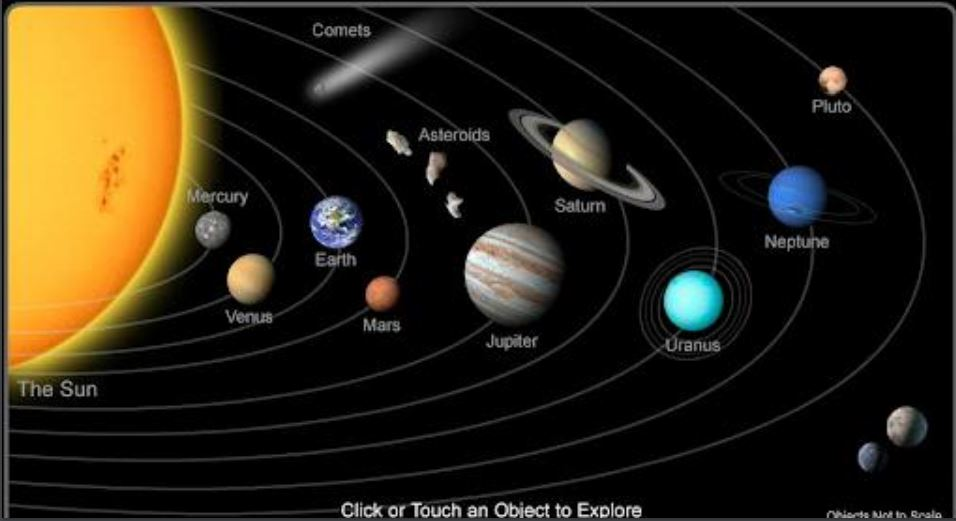
\includegraphics[width=8cm]{2dic/Sistema_Solare.jpg}
    %\caption{Sistema solare}
    \label{fig:SistSol}
\end{figure}

Curiosità: le costellazioni (cioè gruppi di stelle) dello "Zodiaco" sono quelle attraversate dal moto apparente del sole.

\subsubsection{Modelli planetari}

\begin{minipage}{0.295\textwidth}
    \begin{figure}[H]
        \centering
        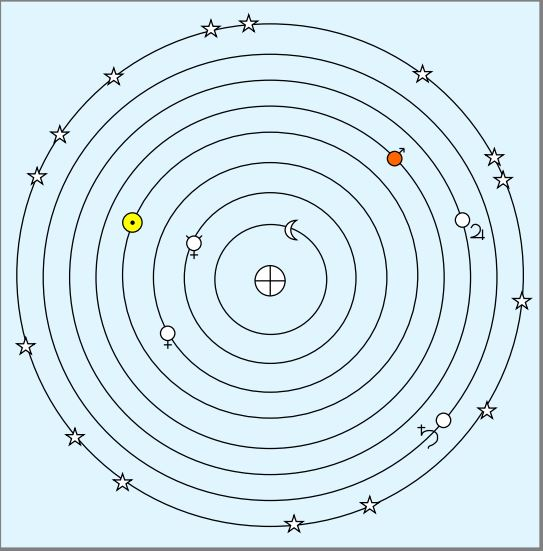
\includegraphics[width=4cm]{2dic/Modello_Planetario_Eudosso.jpg}
        %\caption{Modello planetario ipotizzato da Eudosso (410 a.C.)}
        \label{fig:MPE}
    \end{figure}
\end{minipage}
\begin{minipage}{0.6\textwidth}
    Inizialmente si pensava che la Terra fosse al centro del sistema planetario, ferma, e che fossero invece il sole e gli altri pianeti a ruotare attorno alla Terra, questa visione però cozzava con la presenza di oggetti che sembravano non avere un moto circolare ma che avessero, a volte, anche un moto retrogrado: la loro esistenza fece cadere questa visione iniziale in cui la Terra stava "al centro" (410 a.C, modello di Eudosso).
\end{minipage}

\begin{minipage}{0.295\textwidth}
    \begin{figure}[H]
        \centering
        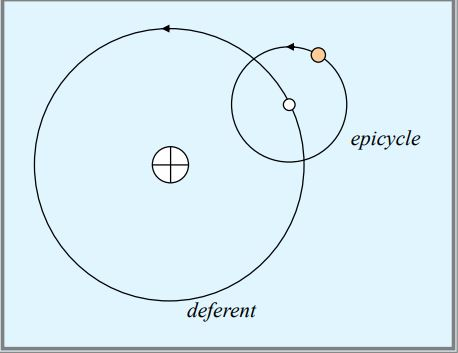
\includegraphics[width=4cm]{2dic/Modello_Planetario_Tolomeo.jpg}
        %\caption{Modello planetario ipotizzato da Tolomeo}
        \label{fig:MPT}
    \end{figure}
\end{minipage}
\begin{minipage}{0.6\textwidth}
    La successiva teoria fu quella di Tolomeo, in cui la Terra stava sempre al centro ma per spiegare i moti retrogradi ipotizzò l'esistenza di epicicli: il centro dell'epiciclo ruotava attorno alla Terra ed alcuni corpi invece ruotavano attorno all'epiciclo. Anche questa teoria non funzionava: non si riuscivano a spiegare i dettagli a meno che l'epiciclo non ruotasse attorno ad un punto che NON era la Terra.
\end{minipage}

\begin{minipage}{0.295\textwidth}
    \begin{figure}[H]
        \centering
        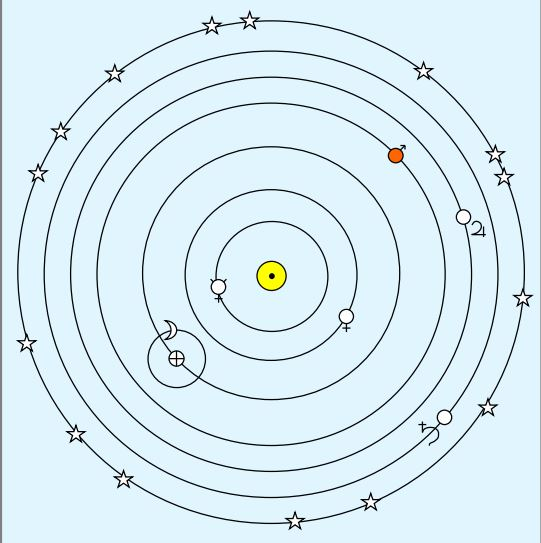
\includegraphics[width=4cm]{2dic/Modello_Eliocentrico.jpg}
        %\caption{Modello planetario eliocentrico}
        \label{fig:MPE}
    \end{figure}
\end{minipage}
\begin{minipage}{0.6\textwidth}
    Nel 1500 abbiamo finalmente una visione eliocentrica: abbiamo il Sole al centro; rimane però il problema della Luna, la quale non gira attorno al Sole ma attorno alla Terra.
\end{minipage}

\subsubsection{Leggi di Keplero}
Fino ad ora abbiamo dato una visione descrittiva, cerchiamo ora anche di dare una visione quantitativa: ci pensò Keplero che introdusse le famose "leggi di Keplero":

\begin{enumerate}
    \item "L'orbita descritta da un pianeta è un'ellisse ed il Sole occupa uno dei fuochi".

    \begin{figure}[H]
        \centering
        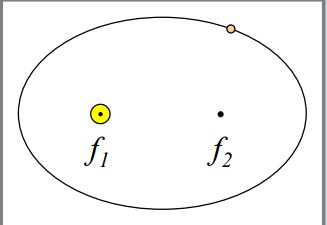
\includegraphics[width=5cm]{2dic/1LeggeKeplero.jpg}
        %\caption{Prima legge di Keplero in cui si vede il Sole occupare uno dei fuochi}
        \label{fig:1k}
    \end{figure}

    \item "Il segmento che unisce il centro del sole con il centro di un pianeta, spazza aree uguali in tempi uguali". Di fatto questa legge rappresenta la conservazione del momento angolare: se l'oggetto è in prossimità del Sole la velocità dell'orbita aumenterà.

    \begin{figure}[H]
        \centering
        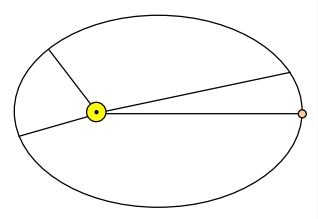
\includegraphics[width=5cm]{2dic/2LeggeKeplero.jpg}
        \label{fig:2k}
    \end{figure}

    \item "I quadrati dei tempi che i pianeti impiegano a percorrere le loro orbite sono proporzionali al cubo del semiasse maggiore.".

    \begin{figure}[H]
        \centering
        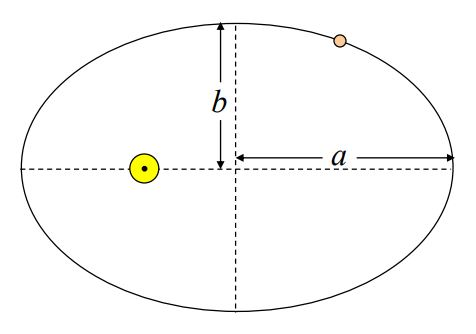
\includegraphics[width=5cm]{2dic/3LeggeKeplero.jpg}
        %\caption{}
        \label{fig:3k}
    \end{figure}
\end{enumerate}

\subsection{Il Sole: struttura interna}
Ma cos'è effettivamente il Sole? Il Sole è il risultato dell'integrazione delle equazioni di struttura stellare e come con tutte le stelle abbiamo fatto delle assunzioni per risolverle: abbiamo detto ad esempio che il Sole non ruota, che non ha campi magnetici, che ha pressione e temperatura pari a zero in superficie.

Tutte queste in realtà non sono vere e rendono il Sole un oggetto molto più complicato di quello che abbiamo descritto nella rappresentazione precedente; tuttavia tale rappresentazione in realtà funziona, perché spiega, negli aspetti fondamentali, la struttura e le condizioni della stella (dimensione, luminosità e temperatura) scelta la massa.

Bisogna quindi tenere a mente che il Sole è più complesso, cioè esso effettivamente ha un suo campo magnetico, ruota e non è una sfera uniforme nella sua "distribuzione di luminosità". Cerchiamo allora di vedere com'è fatto effettivamente il Sole e quali sono le sue proprietà.

Dalle equazioni della struttura, abbiamo concluso che all'interno esiste un nucleo radiativo (con temperature dell'ordine di 15 milioni di gradi) dove si svolgono le reazioni termonucleari tramite la catena PP. Vengono emessi poi fotoni, dunque energia, che si propaga verso l'esterno in una regione detta radiativa, per terminare nella parte più esterna detta zona convettiva.

Ecco alcuni dati del Sole:

\begin{center}
    \begin{tabular}{ll}
        Diametro & $1.4 \times 10^6 \, \text{km} = 109 D_{\rm Terra}$\\
        Massa & $2.0 \times 10^{30} \, \text{kg}=333000 \, M_{\rm Terra}$\\
        Densità & 1400 $\rm kg/m^3$ (160000 $\rm kg/m^3$ al centro)\\
        Temperatura & 5800 K (superficie), $1.55 \times 10^{7}$ K (centro)\\
        Luminosità & $3.86 \times 10^{26}$ W\\
        Tempo di rotazione & 25 giorni (equatore), 35 giorni (poli)\\
        Composizione & 74\% H, 25\% He, 1\% altri elementi\\
        Periodo orbitale & $220 \times 10^6$ anni\\
    \end{tabular}
\end{center}

\subsection{Il Sole: struttura esterna}
Vediamo ora quali sono i fenomeni che accadono effettivamente sulla superficie del Sole e che lo rendono molto diverso da quello che abbiamo assunto.
\subsubsection{Granulazione}
Un primo fenomeno molto interessante è quello della granulazione, cioè il Sole in superficie non appare come una superficie liscia, ma appare come una superficie ricoperta di bolle di gas (dette appunto granuli), che hanno una componente di velocità verso l'esterno (oppure verso l'interno). Queste bolle di gas sembrano essere il risultato di tali moti che portano ad un aumento del livello della superficie (oppure ad una diminuzione).

Questi fenomeni vengono interpretati assumendo che all'interno della stella ci siano delle oscillazioni, cioè si immagina che la struttura autogravitante che è il Sole abbia una sua posizione di equilibrio che può essere perturbata, dando appunto luogo a delle oscillazioni. L'origine di ogni oscillazione è legata ad una forma di richiamo. All'interno del Sole tali forze possono essere o quelle gravitazionali o quelle di pressione.

Quello che si fa è studiare le variazioni luminose del Sole (globalmente o localmente) oppure studiare localmente le variazioni di velocità radiale di queste bolle. Facendo ciò, tramite inversione dei dati ed imponendo alcune condizioni (ad esempio: come deve essere distribuita la materia all'interno del Sole affinché si abbia un'onda stazionaria di un certo), si riesce ad avere una visione che conferma la struttura interna che noi abbiamo determinato risolvendo le equazioni.

Nota: tale descrizione è effettuata mediante sviluppo in armoniche sferiche (come l'atomo di idrogeno).

\begin{figure}[H]
    \centering
    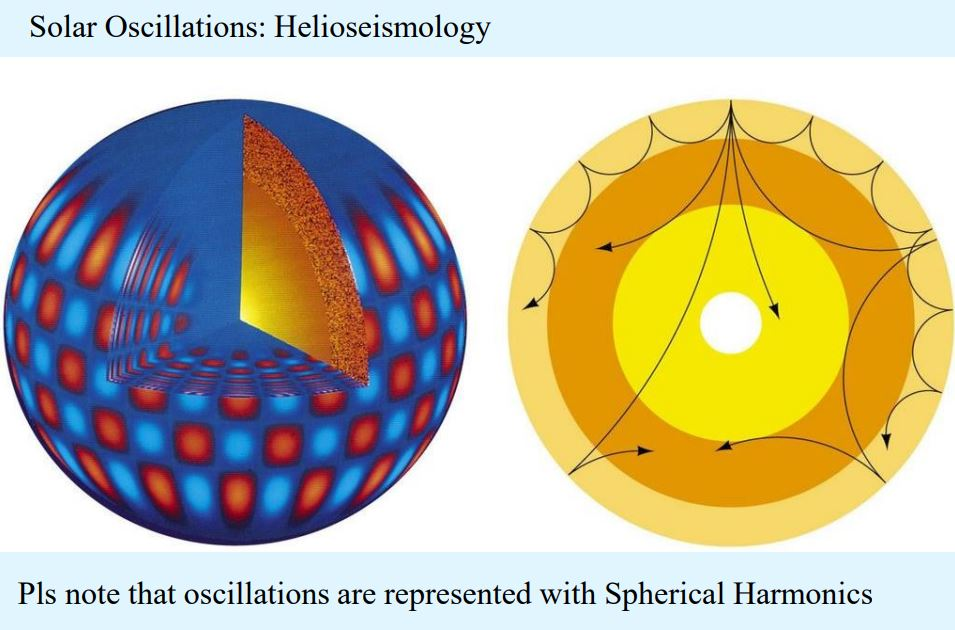
\includegraphics[width=8cm]{2dic/Eliosismologia.jpg}
    \label{fig:Eliosism}
\end{figure}

(In figura: Sviluppo in armoniche sferiche delle oscillazioni delle bolle di gas.)

Ricordiamo che risolvendole abbiamo ottenuto un andamento in funzione del raggio di temperatura, densità e luminosità. La propagazione delle onde dipende dalla densità e l'andamento della densità all'interno del Sole, attraverso lo studio delle onde (che sono stazionarie all'interno) è stato utilizzato per perfezionare il modello del Sole stesso. Questa parte dell'astrofisica si chiama eliosismologia (se in generale applicata alle stelle di parla di astrosismologia). \E possibile misurare le variazioni di luminosità o di velocità radiale nel tempo. Nel caso del Sole si parla di variazioni dell'ordine di 6 minuti, che è il periodo di granulazione; tuttavia si sovrappongono diversi periodi di granulazione che modulano i picchi. L'inversione di questi dati sulla base di armoniche sferiche restituisce l'andamento della densità all'interno del Sole.

\vspace{0.2cm}La parte del sole che noi vediamo si chiama \textit{fotosfera}. Essa non è una superficie omogenea: la luminosità cala dal centro del disco al bordo (oscuramento al bordo), ciò è legato al trasferimento della radiazione in un ambiente curvo, per cui al centro cui l'opacità $\tau$ raggiunge valore 1 ad un profondità fisicamente minore rispetto ai bordi, dove la temperatura è più bassa. 

\textbf{controlla}Risolvendo le equazioni di struttura stellare sappiamo che la temperatura da cui proviene la totalità della luce è di 4500 K; l'ultimo strato da cui vediamo provenire luce ha un temperatura di 7600 K. La larghezza della fotosfera è di 500 km

\begin{figure}[H]
    \centering
    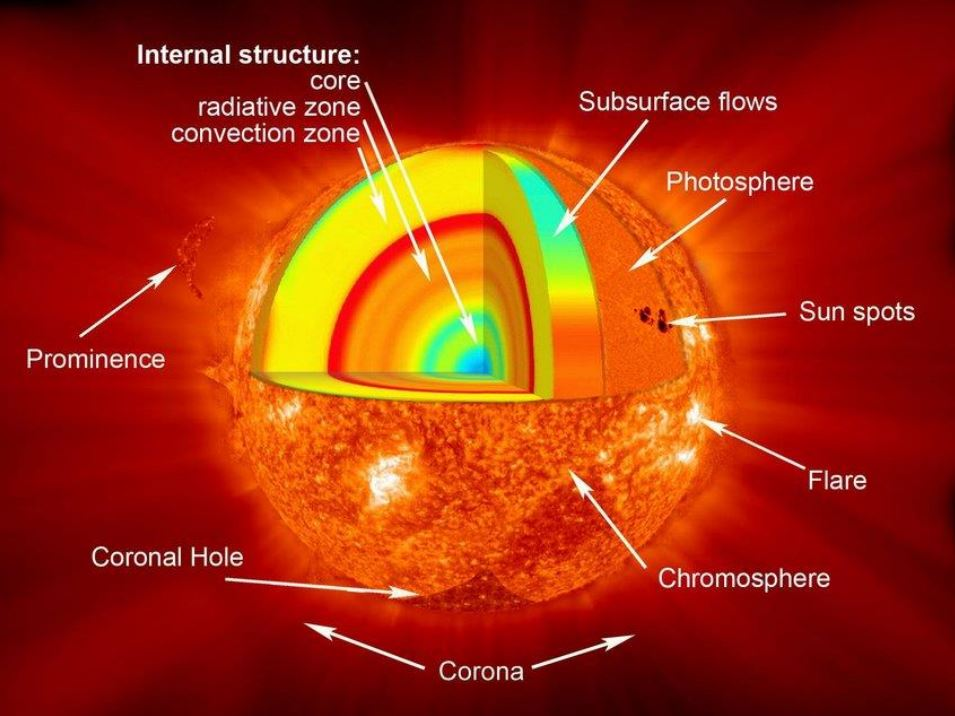
\includegraphics[width=8cm]{2dic/StrutturaSole.jpg}
    \label{fig:StruttSole}
\end{figure}

\subsubsection{Macchie solari (Sunspots)}
Un fenomeno che ancora non è stato spiegato è la presenza sulla superficie di "macchie" solari; esse sono delle regioni che sono più scure. Non è semplice a priori stabilirne la causa, infatti esse potrebbero essere date dal fatto che in quella zona viene bloccata più luce, oppure dal fatto che quella zona è più fredda; quello che possiamo fare è determinare i parametri fisici di una macchia solare, facendo ad esempio lo spettro di tale regione: da questo scopriremo che la macchia appare più scura solo perché è più fredda, non impedisce il passaggio della luce per qualche motivo.

Queste macchie si muovono sulla superficie, questo introduce il concetto di \textbf{rotazione} del Sole: noi interpretiamo gli spostamenti delle macchie solari come un effetto della rotazione solare, cioè immaginiamo che la macchia sia "ancorata alla superficie" e che questa ruoti.

Lo studio del fenomeno è complicato dal fatto che le macchie non sono permanenti nel tempo ma variano la loro forma, dunque non è nemmeno semplice riconoscerle (si pensi al fatto che le macchie impiegano circa 2 settimane ad attraversare il disco visibile, poi passano dall'altro lato e non le possiamo seguire). Si è osservato inoltre che, in un periodo di 11 anni, cambia la numerosità della macchie (nel 1996 ad esempio il Sole non ne presentava nemmeno una!), il cui numero aumenta fino a raggiungere un massimo per poi diminuire nuovamente.

\begin{figure}[H]
    \centering
    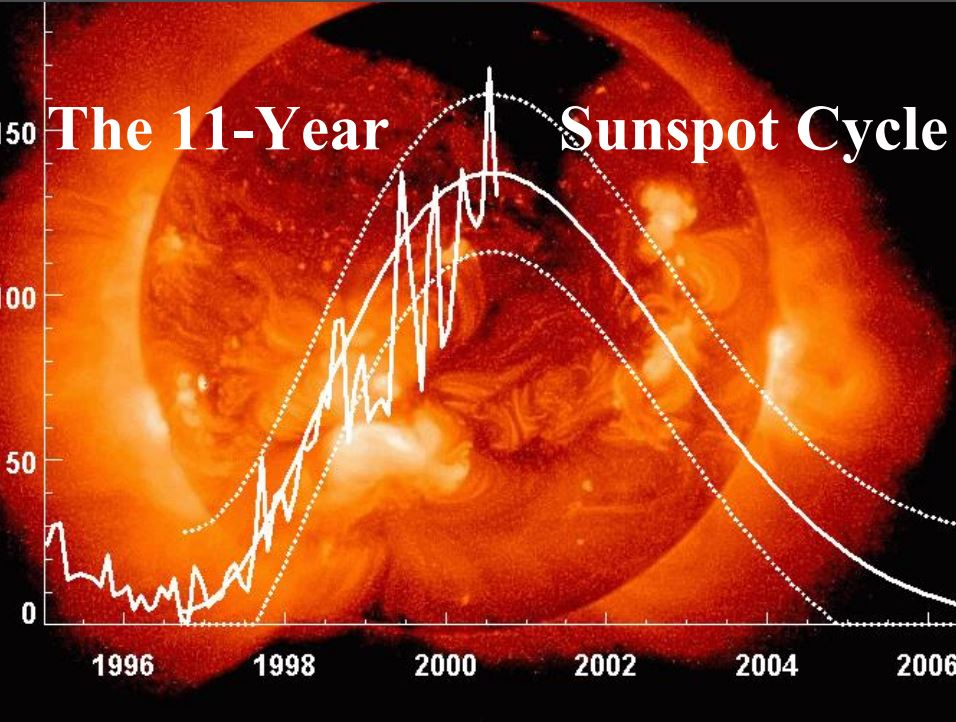
\includegraphics[width=8cm]{2dic/Ciclo11Anni.jpg}
    \label{fig:Ciclo11}
\end{figure}

(In figura: Ciclo di 11 anni delle macchie solari)

Durante tale ciclo di tempo non cresce solo il numero di macchie, bensì anche il luogo dove le macchie si formano. All'inizio di un ciclo, le poche macchie restanti sono molto alte in latitudine (sia Nord che Sud), e le nuove macchie si formeranno a latitudini sempre più basse, fino a formarsi vicino all'equatore (si è raggiunto il massimo?).

\E da notare che ogni 11 anni non si ripresentano sempre lo stesso numero di macchie, esiste dunque una modulazione di più grande durata.

Queste macchie inoltre hanno un impatto sull'atmosfera terrestre però non in maniera diretta in quanto la macchia è il risultato della riorganizzazione del campo magnetico solare il quale interagisce col campo magnetico terrestre e in qualche modo altera l'andamento del clima sulla Terra. Su tempi di scala brevi questo fenomeno non è facilmente visualizzabile.

Quello che però possiamo osservare è nel periodo che va dal 1650 al 1700 il Sole fu privo di macchie e nel corrispondente periodo in Europa ci fu una "piccola" glaciazione.

\E stato anche mostrato che questa attività solare è relazionata al prezzo del grano: pare che i raccolti siano più o meno ricchi a seconda della numerosità delle macchie solari.

Quanto è grande una macchia solare? Ess hanno dimensioni diverse ovviamente, ma in media sono grandi circa quanto la Terra ed è costituita da una regione centrale scura che prende il nome di "ombra" ed una regione circostante che prende il nome di "penombra".

\begin{minipage}{0.45\textwidth}
    \begin{figure}[H]
        \centering
        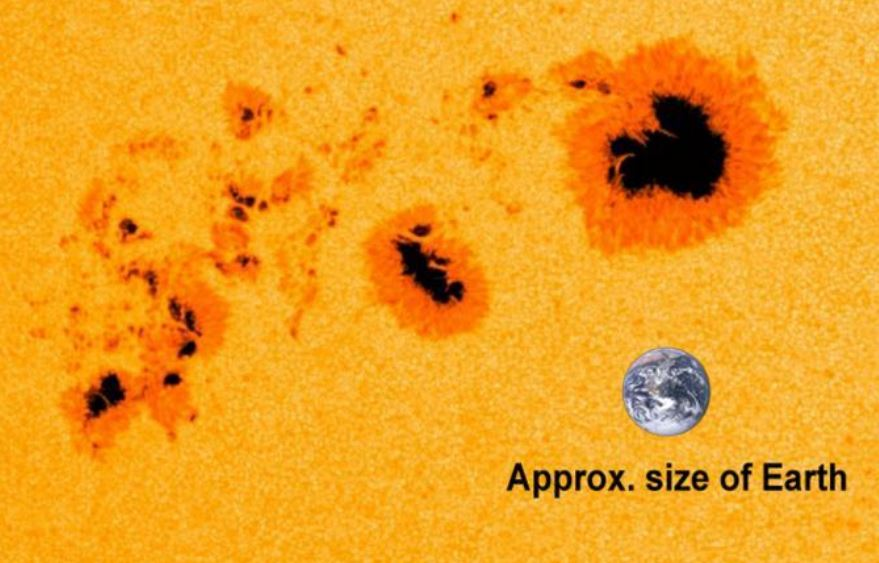
\includegraphics[width=7cm]{2dic/FormaeDimensioneMacchia.jpg} 
    \end{figure}
\end{minipage}
\begin{minipage}{0.55\textwidth}
    \begin{figure}[H]
        \centering
        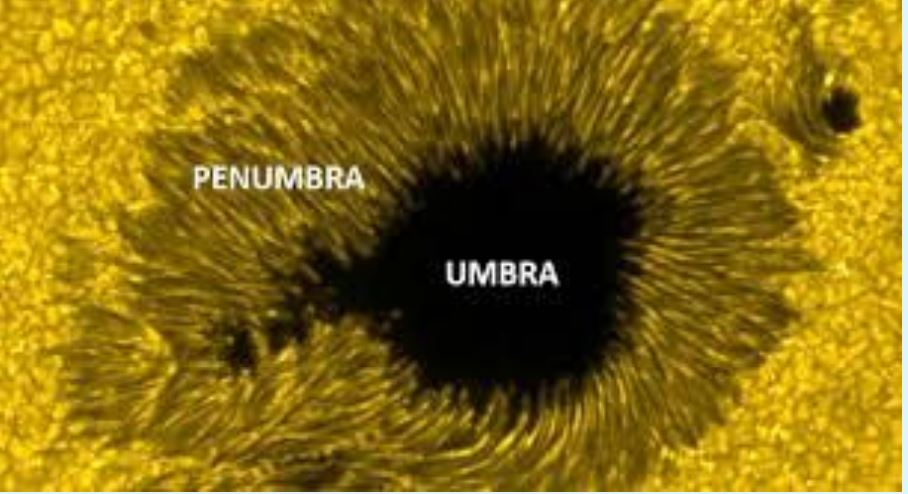
\includegraphics[width=8cm]{2dic/ZoneMacchia.jpg}
    \end{figure}
\end{minipage}

\vspace{0.2cm}(In figura: Dimensioni e regioni delle macchie solari.)

Se confrontiamo ora lo spettro della fotosfera con quello di una macchia solare si vede che esiste una "ragionevole" coincidenza delle linee spettrali ma non sono identiche.

L'interpretazione di tali linee spettrali in termini di temperatura ci dice che la temperatura della macchia è più bassa di quelle dell'ambiente circostante: si scopre che la temperatura della fotosfera è di circa 5800 K, mentre quella della macchia è di circa 4000 K nella zona d'ombra e di 4500 K nella zona di penombra.

Come accade questo? Cos'è che impedisce al calore di diffondersi nella zona della macchia?

Quello che bisogna considerare è il fatto che all'interno di una macchia sono presenti intensi campi magnetici (Hale nel 1908 si occupò di misurare tali intensità dei campi magnetici).

Reminder: se abbiamo una riga spettrale che si forma in un plasma, essa ha una forma caratteristica, per cui se facessimo un grafico flusso-lunghezza d'onda si avrebbe un andamento tale che in corrispondenza di una transizione atomica i fotoni vengono sottratti al flusso, creando una riga spettrale che abbiamo associato ad esempio alla pressione del gas o alle collisioni (allargamenti collisionali delle righe), per cui la riga ha una sua larghezza.

Cosa accade se questa riga si forma in un plasma dove esiste un campo magnetico?

Il metodo usato oggi per misurare il campo magnetico in una stella è quello della spettroscopia in luce polarizzata sfruttando l'effetto Zeeman.

\textbf{riscrivi}

\textbf{Effetto Zeeman} (in breve): se mettiamo degli elettroni (i quali sono dotati di spin) in una regione sede di un campo magnetico succede che, in qualche modo, gli spin degli elettroni si devono allineare col campo; ciò da origine alla suddivisione di un livello energetico in una serie di sottolivelli; il caso più semplice è che si divida in 3 sottolivelli. In conseguenza a ciò, anziché avere una sola transizione che portava alla formazione della riga spettrale adesso ne avremo tre, per cui ora ogni riga spettrale si separa in 3 righe (in realtà non per forza 3, la cosa è più complessa), dunque ora invece di avere una sola transizione ne abbiamo 3 e la separazione $\Delta \lambda$ che si ha tra le linee spettrali è proporzionale al campo magnetico.

\begin{figure}[H]
    \centering
    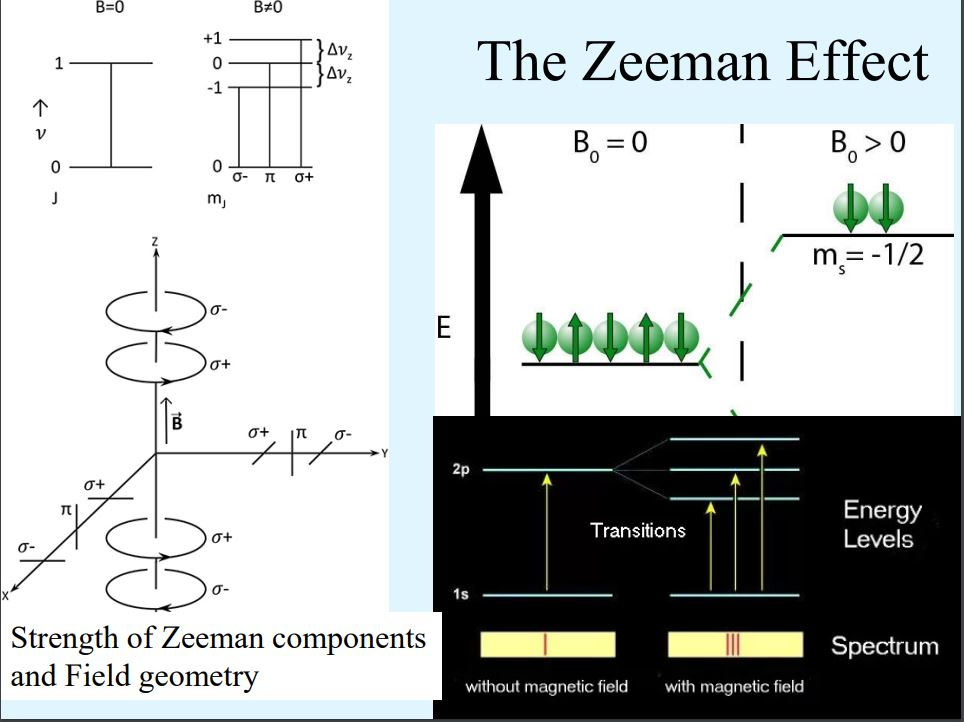
\includegraphics[width=11cm]{2dic/Effetto_Zeeman.jpg}
    \caption{Effetto Zeeman}
    \label{fig:Zeeman}
\end{figure}

Grazie a tale effetto è possibile misurare campi magnetici.

Grazie alla spettroscopia nel 1908 Hale scoprì che queste zone erano magnetizzate. Con la tecnologia odierna si riescono a vedere tutte le singole parti della macchia, e siccome le proprietà polarimetriche\footnote{Le proprietà polarimetriche si riferiscono alla capacità di un oggetto o di un sistema di influenzare la polarizzazione di un'onda elettromagnetica incidente.} delle componenti sono legate alla geometria del campo, è possibile misurare anche la direzione del campo, oltre l'intensità. Se facciamo questo, scopriamo che nella macchia è presente una zona di ombra con un campo sostanzialmente verticale, il quale si inclina sempre più man mano che proseguiamo verso la zona di penombra (vedi figura).

Hale inoltre scoprì che le macchie nascevano sempre a coppie e che la polarità del campo nella coppia di macchie era inversa, cioè da una macchia si aveva un campo positivo mentre nell'altra era negativo (cioè le linee di campo emergono da una macchia e entrano nell'altra).

\begin{figure}[H]
    \centering
    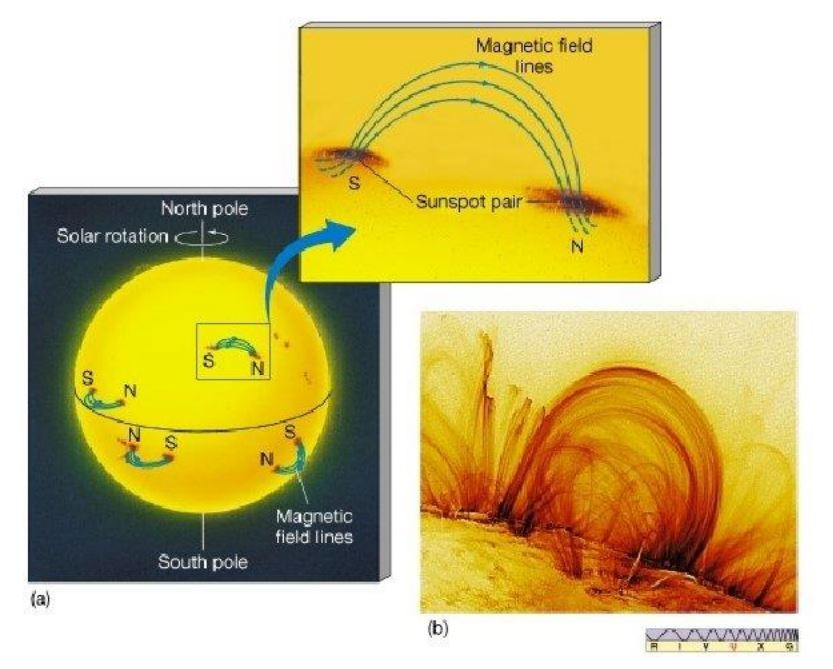
\includegraphics[width=11cm]{2dic/CampiMagneticiMacchie.jpg}
    \label{fig:CampoMag}
\end{figure}

Dunque possiamo affermare che le macchie "emergono" sempre in coppie ed hanno la loro polarità. Con la tecnologia attuale si può anche vedere l'andamento del campo magnetico che emerge da una macchia e rientra in un'altra; infatti in realtà le linee di campo sono dei veri e propri "tubi" di campo, all'interno del quale può fluire la materia. Se quindi il campo dà origine ad un contenimento del plasma, il plasma all'interno si troverà ad una densità diversa da quella ambientale, e ciò sarà visualizzabile con una immagine "in luce" dove questo plasma emette, cioè possiamo fotografare il Sole utilizzando un filtro che seleziona la radiazione in corrispondenza dell'emissione della riga H-$\alpha$ dell'idrogeno, e in questo modo tracciamo il plasma che si muove all'interno dei tubi di campo magnetico.

Ma perché queste regioni sono più fredde?

Istintivamente si potrebbe pensare che siccome sulla fotosfera si ha una pressione di gas che compensa il peso degli stati sovrastanti, e siccome nelle macchie si hanno dei campi magnetici, i quali generano pressione, la pressione del gas si abbassa ed essendo questa proporzionale alla temperatura si abbassa quest'ultima, ma non è così.

Il fatto è che all'interno della fotosfera esistono dei fenomeni di convezione, che consistono in uno spostamento di materia ionizzata. Nel momento in cui siamo in presenza di un campo magnetico, tale materia viene deflessa, dunque si spegne la convezione. Se si spegne la convezione, la quale è il sistema più efficiente di trasporto di energia e di calore, il flusso di calore proveniente dagli strati più bassi e che deve attraversare gli strati sovrastanti incontra maggiore difficoltà nelle zone delle macchie ed il plasma dunque appare più freddo.

\begin{figure}[H]
    \centering
    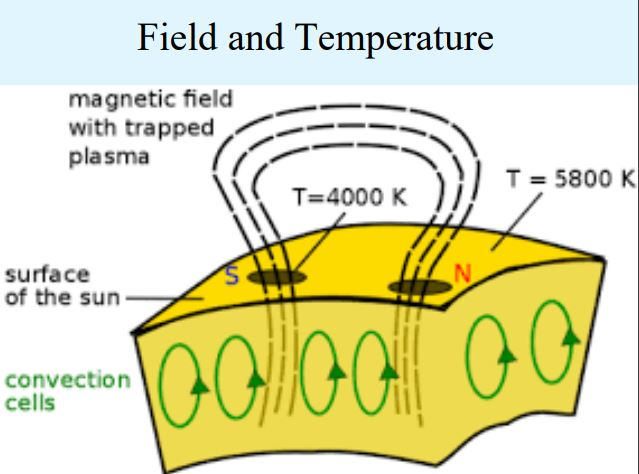
\includegraphics[width=8cm]{2dic/ConvezioneMacchie.jpg}
    %\caption{Come il campo magnetico interferisce col fenomeno della convezione}
    \label{fig:Convezione}
\end{figure}

Ricapitolando, tra due macchie, che sono regioni in cui si ha evidenze di campi magnetici, si ha un collegamento perché si ha un campo magnetico che riemerge e poi rientra, ciò viene visualizzato dal plasma intrappolato dal campo magnetico. A tali strutture è stato attribuito il nome di filamenti e prominenze.

Il plasma ferma la radiazione dietro, la quale anziché passare viene assorbita creando quindi una zona scura, oppure quando si staglia fuori dal disco solare appare brillante \textbf{che cazzo vuol direeeee, è collegato ai due nomi}

Le prominenze assumono dimensioni gigantesche, fino a un quinto del disco solare.

La domanda è ora da dove viene il campo magnetico?

La situazione è molto complicata perché subentrano tutta una serie di fenomeni riguardo l'origine del campo magnetico e su come questo possa dare origine alle macchie.

Affrontiamo il primo problema. Il campo in una stella può essere presente sostanzialmente per due motivi:

\begin{enumerate}
    \item C'era già nella nube da cui la stella si è formata (ricordiamo che una nube è ampia 7 mila anni luce, per cui anche se il campo fosse debole localmente nel momento in cui la nube si compatta può venire fuori un campo molto grande); però il campo potrebbe comunque dissiparsi (come succede ad esempio nei magneti permanenti: essi non durano all'infinito);
    \item Potrebbe essere generato creando una corrente elettrica che nel Sole è data dai moti di convezione, dando vita ad una sorta di "processo dinamo", che nel Sole è detta appunto "dinamo solare". Nel cercare di creare un modello di campo magnetico per la dinamo solare subentrano molte complicanze: innanzitutto noi vediamo solo quello che "avviene fuori" quindi non sappiamo di preciso tutto quello che invece avviene dentro. Quello che serve in un modello di dinamo è che bisogna generare sia la componente radiale che quella tangenziale del campo. Se generassimo il campo con una corrente, esso avrebbe solo una componente ortogonale alla superficie, e inoltre tale campo tenderebbe a impedire la circolazione della corrente.
    
    Nel caso della stella, il motore è la necessità di spostare energia dal centro verso l'esterno, ed esso deve esistere altrimenti la stella esploderebbe, ci vuole quindi un equilibrio tra la convezione che genera il campo e il campo che blocca la convezione. Nel caso del Sole tale campo incontrerebbe il fenomeno detto "rotazione differenziale" cioè il Sole non ruota come un corpo rigido, ma esso ruota più velocemente all'equatore di quanto non faccia ai poli ed il tutto diventa più complicato perché la materia nel moto "trascina con sé" il campo. Ci possono essere due regimi: uno in cui il campo blocca la materia e uno in cui la materia nel suo muoversi trascina il campo (come se il campo fosse "congelato" con la materia). \textbf{ULTRA CHIEDI A MARIKA}

    In questo secondo caso accade che la materia produce una deformazione del campo e si ha la creazione di spire. Qui interviene la convezione ciclonica, la quale fa sì che tali spire, oltre ad avvolgersi nel verso di rotazione, possano dare origine a dei loop (orientati lateralmente alla superficie, verso l'esterno \textbf{sicuro?}) e qui si può avere l'emersione del campo rispetto alla superficie, dando origine alle macchie.
\end{enumerate}

%Nota: Il risultato finale nasce dalla creazione di campi in punti diversi della stella. Tale risultato ha però come effetto di bloccare il moto della materia, ma la materia non si può bloccare perché l'energia deve uscire. Questo è il motivo per cui si ha una ciclicità nella comparsa delle macchie ogni 11 anni: tale tempo è il temp necessario per fermare tutto per poi ricominciare

\begin{figure}[H]
    \centering
    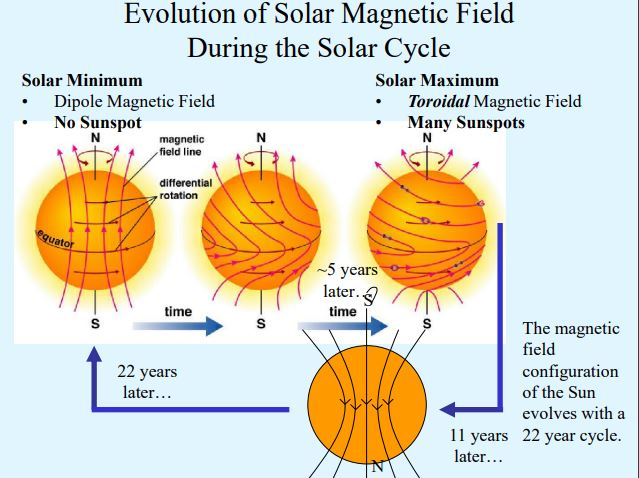
\includegraphics[width=11cm]{2dic/RotazioneDifferenziale.jpg}
    \label{fig:CampiMageRotazDiff}
\end{figure}

\subsubsection{Effetti della rotazione differenziale}

Quello che la rotazione differenziale ci offre è un campo magnetico periodico.

Possiamo anche considerare il fenomeno della rotazione differenziale in relazione al fenomeno delle oscillazioni e studiare le oscillazioni delle bolle di gas a latitudine diversa, per cercare di capire dove è l'origine della rotazione differenziale stessa, dato che essa è fondamentale per la generazione del campo magnetico.

Dato che le oscillazioni danno la possibilità di studiare l'interno del Sole, ci poniamo il problema di capire come cambia la velocità di rotazione con gli strati.

La risposta sta nella figura che segue:

\begin{figure}[H]
    \centering
    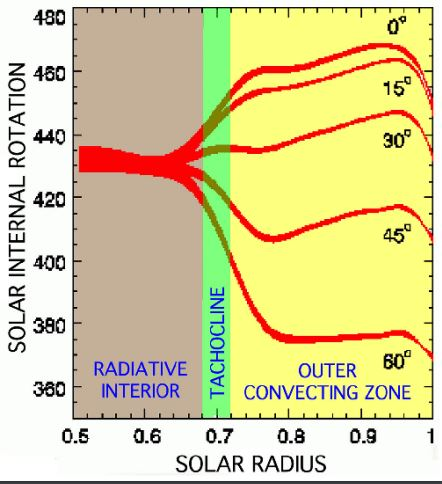
\includegraphics[width=8cm]{2dic/Tachocline.jpg}
    \caption{Velocità di rotazione in funzione del raggio a diverse latitudini}
    \label{fig:VelRotDiff}
\end{figure}

In essa si vede qual è la rotazione al variare della latitudine, negli strati più interni.

Il risultato dell'inversione dei dati ricavati dalle oscillazioni è che gli strati più interni all'equatore si muovono più velocemente, mentre ad alte latitudini la velocità diventa più bassa; tutto questo sembra avere a che fare con la zona convettiva, poi tutte le velocità si riuniscono in una zona ed assumono lo stesso valore, indipendentemente dalla latitudine, tale zona è detta "tachocline".

Quindi il Sole ha una rotazione differenziale che coinvolge solo gli strati più interni. Ciò porta a pensare che la generazione del campo sia legato alla regione convettiva.

Cosa può succedere al campo magnetico nel tempo?

Quando nel 1996 non erano presenti macchie possiamo pensare che il campo magnetico fosse puramente dipolare. Sappiamo infatti che il campo magnetico può essere sviluppato in serie di multipoli; se tutti i termini superiori a quello dipolo fossero nulli non avremmo macchie perché il campo magnetico sarebbe tutto all'interno della stella e poi emerge solo radialmente.

Tale campo magnetico sarebbe comunque dell'ordine di 2 Gauss, dunque non avrebbe effetti sul fenomeno della convezione (non riesce ad alterare il moto della materia), perché di intensità molto bassa.

Nel tempo, a causa della rotazione differenziale, appare una componente toroidale, dunque trasversa, del campo magnetico; questo fenomeno ha una durata di 22 anni.

Tale durata è legata al ciclo delle macchie di 11 anni di cui abbiamo parlato prima, si è scoperto infatti che passati 11 anni riappaiono le stesse macchie ma con polarità invertita. Dunque tenendo conto della polarità il reale ciclo è di 22 anni.

\subsection{Atmosfera del Sole}
\subsubsection{Temperatura}
La presenza di campi magnetici e della macchie influenzano ovviamente la temperatura dell'atmosfera; osserviamo il grafico seguente:

\begin{figure}[H]
    \centering
    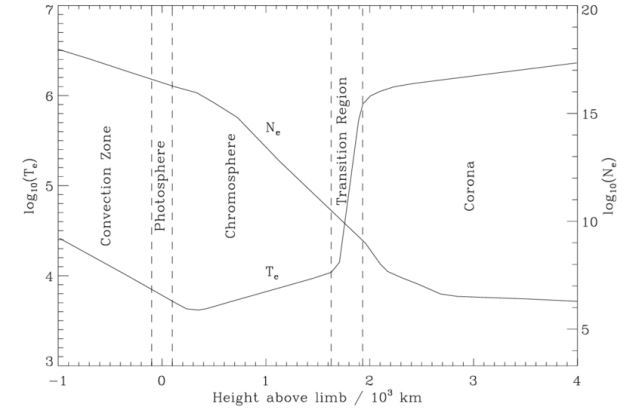
\includegraphics[width=12cm]{2dic/TemperatureAtmosfera.jpg}
    \label{fig:Temp}
\end{figure}

(In figura: Andamento della temperatura e della densità elettronica nell'atmosfera del Sole in funzione dell'altezza dal bordo.)

La temperatura, man mano che aumenta l'altezza, va scendendo, fino alla zona della fotosfera (quella che vediamo noi). Per quanto riguarda la densità elettronica, essa diminuisce perché diminuisce la pressione.

Man mano che guardiamo gli strati più alti dell'atmosfera rispetto alla fotosfera (cioè mentre andiamo all'esterno del Sole) la temperatura comincia a risalire (questo non ci sorprende molto, anche nella Terra succede), tale regione in cui la temperatura comincia a risalire è detta \textit{cromosfera}; poi ad un certo livello in cui la temperatura è sì risalita ma è comunque nell'ordine di dieci mila gradi (e dunque ha un valore non molto diverso da quello iniziale), si ha un aumento della temperatura incredibile: nel giro di qualche centinaio di km la temperatura passa da dieci mila gradi ad un milione di gradi. Tale regione è detta \textit{regione di transizione} ed essa è caratterizzata da densità molto basse. Segue una regione, senza fine, detta \textit{corona} in cui la temperatura aumenta ancora, mentre la densità elettronica scende.

La regione di transizione produce un fenomeno visibile dalla Terra (anche se è rarissimo vederlo), detto "green flash" (che poi di fatto è la cromosfera); esso si osserva quando il Sole tramonta: c'è un momento in cui l'orizzonte taglia la fotosfera e mostra solo la cromosfera, in tale istante si vede una luce verde. Sostanzialmente quello che succede è che a causa delle alte temperatura gli atomi di elio che sono presenti in tale zona si eccitano per collisione e segue un successivo decadimento con emissione di fotone, la cui lunghezza d'onda cade appunto nel verde.

\begin{figure}[H]
    \centering
    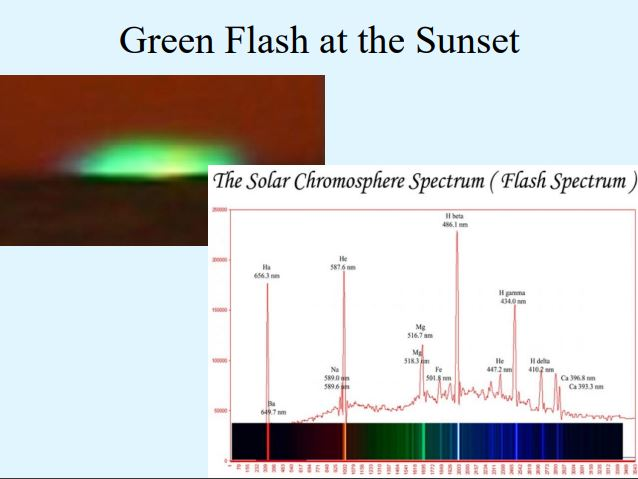
\includegraphics[width=8cm]{2dic/GreenFlash.jpg}
    %\caption{Immagine del Green Flash}
    \label{fig:GF}
\end{figure}

Un altro modo per vedere gli strati più esterni del sole è sfruttando i fenomeni di eclissi che mettono in evidenza gli strati più esterni. In questo modo, anche prima di avere ben chiara la struttura del Sole, si riuscì a capire che gli strati più esterni del Sole erano a temperatura maggiore di quella della fotosfera, ciò sempre grazie alla spettroscopia, infatti in tali strati apparivano righe di atomi altamente ionizzati (come l'elio ad esempio), i quali per ionizzarsi hanno bisogno di altissime temperature.

Oggi esiste uno strumento detto coronografo che permette di "simulare" un'eclissi per vedere gli strati più esterni del sole.

\begin{figure}[H]
    \centering
    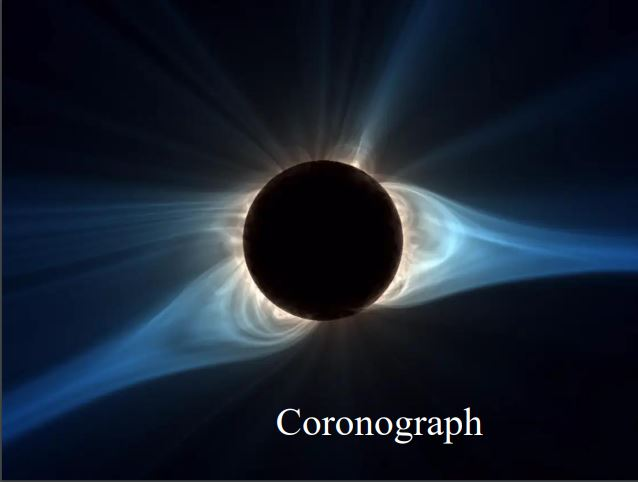
\includegraphics[width=8cm]{2dic/Coronografo.jpg}
    %\caption{Immagine ottenuta mediante un coronografo}
    \label{fig:Coronografo}
\end{figure}

Trivia: quando ci sono eclissi è normale che ci siano nuvole, infatti esse sono dovute al repentino cambio di temperatura dovuto alla mancanza di irraggiamento.

\subsection{Ripasso della lezione precedente}
La volta scorsa abbiamo parlato del Sole e abbiamo osservato che la parte che noi vediamo è la fotosfera (per definizione). Questa fotosfera è caratterizzata da una temperatura che sembra aumentare andando verso l'interno, è dell'ordine di 10000 gradi e scende alla superficie intorno ai 5700.

Questa diminuzione della temperatura con la quota dell'atmosfera non continua, ma si ha un punto di inversione (la temperatura risale e questa zona prende il nome di cromosfera), anche se si ha un cambiamento solo di un fattore 2, mentre si ha una rapidissima caduta della densità elettronica (scende più di un ordine di grandezza). Andando sempre più in profondità la densità elettronica continua sempre a diminuire e la temperatura ad aumentare e si raggiunge uno strato più esterno dell'atmosfera solare, che prende il nome di corona, dove la temperatura è dell'ordine di milioni di gradi, la densità elettronica adesso è scesa a $10^{6} \, \rm el \cdot cm^{3}$.

Cosa ci si aspetta in questi strati di atmosfera più esterni? Dato che le condizioni sono di bassa densità, ci si aspetta che eventuali righe spettrali siano in emissione, perché se i livelli non si depopolano per collisione osserviamo righe in emissione. La depopolazione dei livelli per collisione la rivediamo con una termalizzazione dell'energia del campo elettromagnetico e quindi una temperatura del gas.

Che le righe nella cromosfera siano in emissione si è scoperto da Terra con il green flash: nell'istante in cui il Sole scende sotto l'orizzonte, si ha la possibilità di osservare una regione caratterizzata da un'emissione verde che è dovuta alle righe di transizione dell'elio (il quale è stato scoperto dal Sole, da cui il nome) ed effettivamente in uno spettro della cromosfera troviamo le righe dell'elio e del magnesio, che sono tutte in emissione.

Il fenomeno dell'eclissi ha poi permesso di prendere atto dell'esistenza di uno strato di atmosfera che circonda il disco solare che non ha forma sferica, bensì presenta i cosiddetti "streams". Dall'analisi di quest'ultimi si nota che essi sono governati dalla presenza di flussi di plasma che si muovono lungo tubi che scopriremo essere dovuti al campo magnetico.

Abbiamo detto in precedenza che la presenza di righe spettrali e la loro intensità è funzione della temperatura e abbiamo visto ciò per gli elementi di basso stato di ionizzazione, neutri o per molecole, potendo caratterizzare le atmosfere delle stelle, attribuendo un tipo spettrale. Nel caso del Sole, una spettroscopia degli strati a diversa distanza dal disco solare porta all'andamento della temperatura in funzione della distanza caratterizzato come visto prima. Tutto ciò è stato definito osservando la presenza e l'intensità di righe spettrali che si formano in quelle particolari condizioni.

\begin{figure}[H]
    \centering
    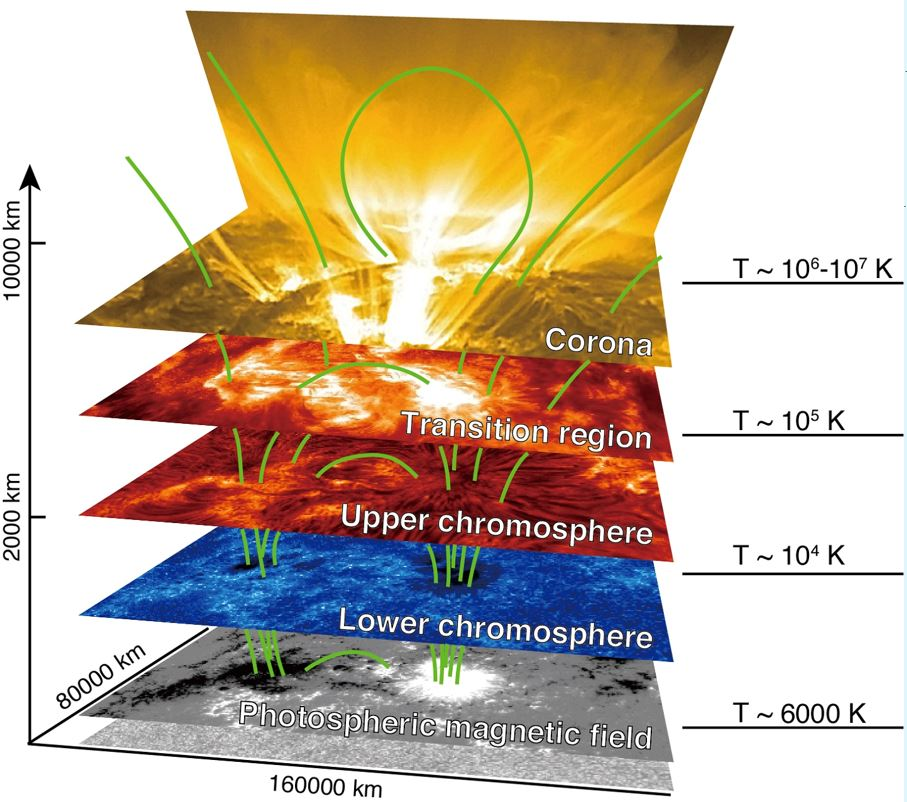
\includegraphics[width=8cm]{Struttura interna del Sole.JPG}
    %\caption{Struttura interna del Sole}
    %\label{fig:Struttura interna del Sole}
\end{figure}

Diamo dettagli in più sui vari strati:

\begin{itemize}
    \item La cromosfera ha una temperatura dell'ordine di 10000 gradi ed è caratterizzata da strutture che prendono il nome di "spicole", che sono dei getti di plasma. Quindi l'atmosfera non si presenta come un oggetto solido, piuttosto come dei getti di materia che hanno la durata di circa 15 minuti e che sono grandi centinaia di km e si muovono con una velocità di 20 km/s. Questo significa che la cromosfera non è un ambiente stabile, bensì è un ambiente continuamente in formazione e disgregazione.
    
    La riga più intensa che riusciamo a vedere di questa cromosfera è la riga dell'H-$\alpha$, che è la riga spettrale della transizione 3-2 dell'idrogeno che possiamo vedere in emissione. Per vedere la cromosfera dobbiamo utilizzare un filtro che produce un'immagine del Sole all'interno di questa banda spettrale;
    \item Nella regione di transizione si ha un elevatissimo incremento di temperatura e pressione ed appare verde poiché a questi valori di temperatura la riga più evidente è quella dell'elio;
    \item La corona è invece caratterizzata da una emissione nell'X e, a differenza degli strati precedenti, possiede una forma più complicata. Per quanto riguarda la visione che noi abbiamo di questi strati, essa viene fuori da una modellistica: sembrerebbe che ci siano degli strati a temperatura diversa che all'analisi appaiano caratterizzati dalla presenza di campi magnetici. I campi magnetici che sono presenti negli alti strati nell'atmosfera solare hanno origine nelle macchie fotosferiche, in una struttura di tipo loop; sembra quindi che man mano che si va all'esterno del Sole la temperatura salga e che la fenomenologia sia legata ai diversi strati, dove il campo magnetico ha strutture diverse e diventa sempre più debole, per cui interagisce con il plasma;
    \item La parte ancora più esterna del Sole, quella che supera la corona, sarebbe la regione non più statico-gravitazionalmente legata al Sole ma quella del cosiddetto vento solare (con vento si intende un flusso di particelle): il Sole in sostanza è circondato da un ambiente dove le particelle cariche si muovono con una simmetria non sferica (a velocità dell'ordine di migliaia di km/s). Lungo l'equatore del Sole vediamo delle strutture di plasma chiamate streams, mentre ortogonalmente queste non sembrano essere presenti però il flusso del vento solare è più alto e la velocità è più alta \textbf{che cazzo vuol dire}.
\end{itemize}

Ma cos'è che dovrebbe provocare questo aumento di temperatura dal basso verso l'alto? Sembrerebbe che alla base ci siano una serie di fenomeni legati o a onde che dissipano energia oppure a fenomeni come la riconnessione magnetica.

I campi magnetici in generale sono la soluzione che invochiamo quando non si capisce il perché di una cosa, ma la magnetoidrodinamica in generale è veramente complicata, ma un teorema che possiamo affrontare è il teorema di Alfven, che è alla base di tanti fenomeni.

\subsection{Teorema di Alfvén}
Questo teorema parte dalle correnti parassite: se abbiamo un magnete e facciamo passare velocemente un metallo dentro, accade che gli elettroni del metallo vedono passare il campo e si ha quindi una variazione del campo nel tempo, per cui viene generata corrente. Queste correnti saranno più intense quanto più il campo è intenso e quanto più velocemente passa l'oggetto.

\begin{figure}[H]
    \centering
    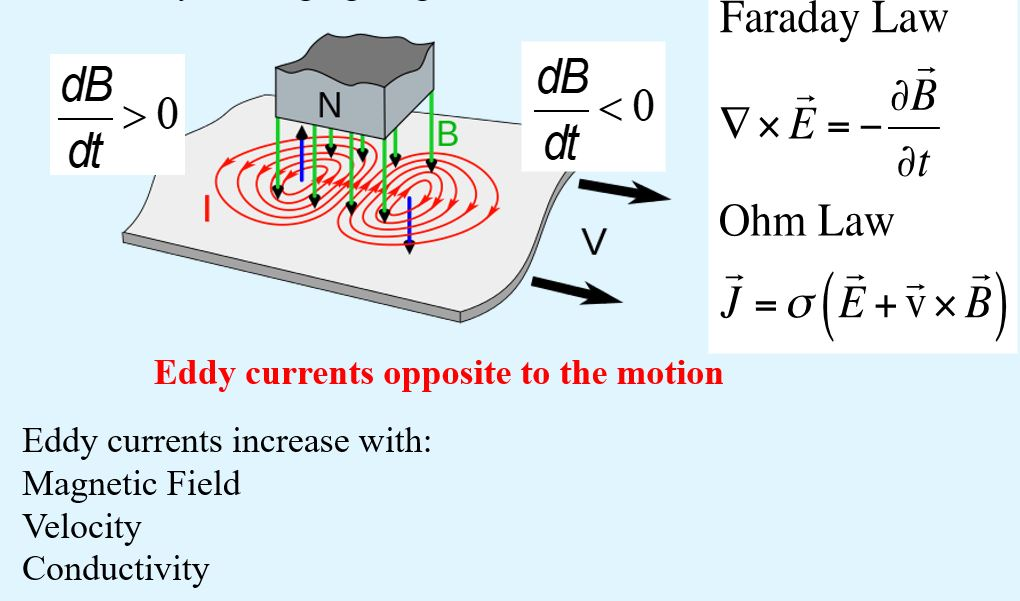
\includegraphics[width=14cm]{Correnti parassite.JPG}
\end{figure}

Supponiamo ora che a scorrere non sia un metallo bensì un plasma. Esso per definizione possiede conduttività infinita in quanto gli elettroni sono liberi di muoversi, perciò dovrebbe generare delle correnti parassite infinite. Questo fu spiegato nel 1942 da Alfven, il quale introdusse questo concetto, concludendo che se si è in presenza di un materiale con conduttività infinita, quando questo si muove si tira dietro il campo (da qui l'espressione "approssimazione di campo congelato", cioè come se il campo fosse congelato con la materia e dovesse muoversi). Se ciò è vero, significa che quando muoviamo in qualche il modo il plasma all'interno di un campo spostiamo l'intero campo.

Possiamo considerare i 2 casi estremi: un plasma con conduttività infinita che si muove e trascina il campo, oppure il caso più ordinario in cui la materia si muove seguendo le linee del campo (il moto della materia è dominato dal campo oppure il campo è dominato dalla materia). Il primo caso potrebbe essere il motivo per cui le celle convettive nel Sole dove incontrano un campo si fermano, riducono la trasmissione dell'energia dal basso verso l'alto e danno origine alle macchie come zone fredde; mentre il secondo è il caso della dinamo solare, cioè quando vediamo l'equatore che si muove più velocemente del polo attorcigliando le linee del campo(aumenta l'intensità del campo e la materia non riesce più a trasportare il campo\textbf{ma si deforma? chiedi a marika}).

Supponendo che questo sia un modello di come al movimento della materia si possa muovere un campo, si spiega il riscaldamento degli strati superiori dell'atmosfera solare attraverso un fenomeno chiamato \textbf{riconnessione magnetica}: esso è un concetto estremamente recente (nel 1950) ed è basata sull'idea che se avessimo 2 plasmi con campo magnetico per esempio inverso e li spingiamo uno contro l'altro, le linee di campo si rompono e si riconnettono (in punti detti punti $x$) per dare origine a un campo magnetico di struttura diversa.

\begin{figure}[H]
    \centering
    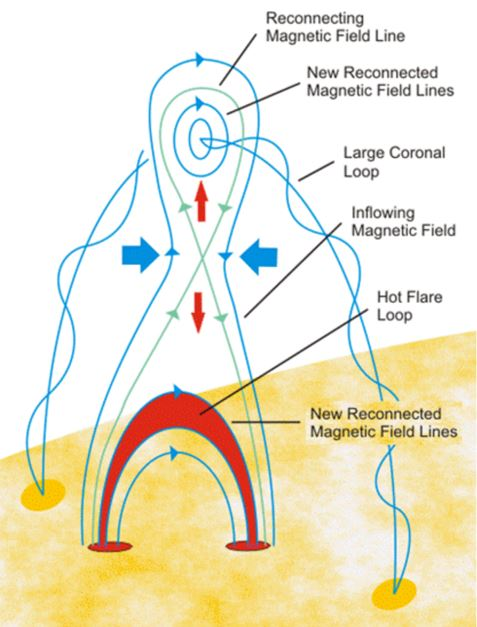
\includegraphics[width=8cm]{Riconnesione magnetica.JPG}
\end{figure}

Quando si riorganizza il campo magnetico, l'energia del campo diventa energia cinetica e le particelle diventano più veloci, facendo aumentare la temperatura.

Oltre la riconnessione magnetica ci sono anche altre forme di riscaldamento più standard come nel caso delle onde la conversione dell'energia dell'oscillazione in energia meccanica, oppure una turbolenza la quale, rispetto ad un flusso laminare, ha una maggiore viscosità, quindi si dissipa energia. 

\subsection{Il sistema solare}
D'ora in poi misureremo tutto in unità astronomiche, che sono all'incirca 150 milioni di km (che è la distanza tra il Sole e la Terra). Le distanze dei pianeti dal Sole in unità astronomiche sono

\begin{figure}[H]
    \centering
    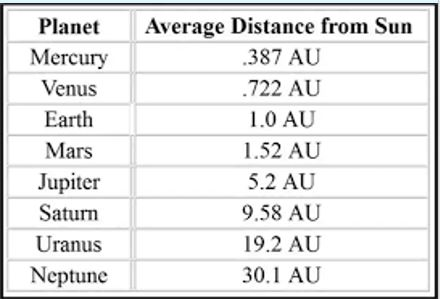
\includegraphics[width=6cm]{Distanze.JPG}
\end{figure}

(trick per ricordarli: se scriviamo i numeri 0,3,6,12,24,48,96 a cui sommiamo 4 e dividiamo per 10 otteniamo tali distanze in maniera grossolana)

Vale la terza legge di Keplero: il periodo al quadrato (espresso in anni) è uguale al cubo della distanza (espressa in unità astronomiche).

La Terra ha un satellite, la Luna, che orbita a una distanza di 400000 km attorno alla Terra, con un orbita quasi circolare (l'eccentricità è praticamente quasi zero); c'è sincronismo: il periodo di rivoluzione è uguale al periodo di rotazione (dura 28 giorni), per cui vediamo sempre la stessa faccia, questo dà origine alle fasi lunari; inoltre il piano orbitale della Luna non è coincidente con quello della Terra (c'è una differenza di 5.2 gradi), il che fa sì che non ci sia un'eclissi al mese (cosa che accadrebbe se l'angolo fosse zero). Il periodo al termine del quale Sole, Terra e Luna si trovano quasi esattamente nella stessa posizione reciproca e possono ripetersi le stesse eclissi lunari e solari è detto \textit{ciclo di saros}, di circa 18 anni.

\vspace{0.2cm}Abbiamo poi i pianeti del sistema solare, che li dividiamo in 2 gruppi:

\begin{itemize}
    \item Pianeti rocciosi, fino a Marte, che hanno una densità tipica dei minerali, cioè tra i 4000 e i 5000 kg/m$^{3}$ e possiedono una piccola atmosfera (piccole rispetto alle dimensioni del pianeta);
    \item Pianeti gassosi.
\end{itemize}

Tutti i pianeti ruotano in senso antiorario tranne Venere che possiede una rotazione retrograda (insieme ad Urano che possiede un asse di rotazione quasi orizzontale), e ciò è legato alle interazioni che ci sono state nelle fasi iniziali tra tutti i corpi che si sono formati\footnote{Se ricordiamo che un sistema solare si forma con una nube che collassa e dà origine al Sole e ai pianeti, ci aspettiamo che tutto dovrebbe girare nello stesso verso in cui girava la nube all'inizio.}.

Le temperature dei pianeti sono mediamente alte, dipendono dalla distanza dal Sole

\begin{figure}[H]
    \centering
    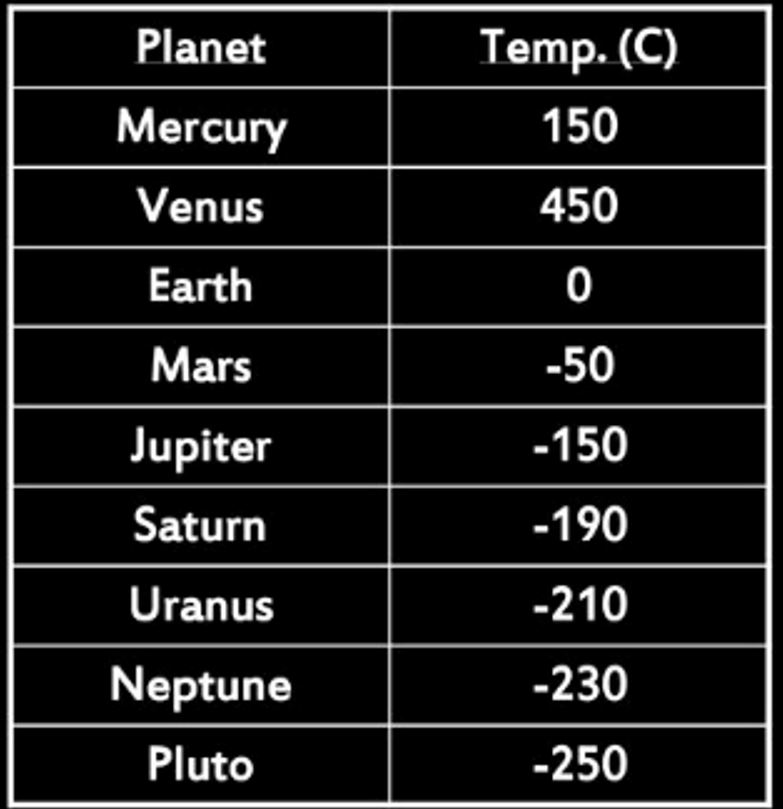
\includegraphics[width=4cm]{Temperature.JPG}
\end{figure}

La composizione chimica dei pianeti è abbastanza simile: nei pianeti interni i contenuti in metallo sono identici, questo fa pensare che si siano formati tutti dallo stesso nucleo iniziale; lo stesso vale per i pianeti più esterni, anche qui le percentuali (stavolta però si parla di gas) sono tutte identiche.

I pianeti più interni (tranne la Terra) non hanno satelliti; Marte ne ha due i quali non hanno forma sferica, per cui probabilmente sono stati catturati dalla fascia degli asteroidi; i restanti pianeti hanno tutti satelliti anche molto grandi (quasi quanti la Terra). I satelliti più famosi sono quelli di Giove (Io, Europa, Ganymede e Callisto) perché essi sono stati la prova dell'esistenza di un sistema solare, dato che riproducevano quest'ultimo in un certo senso.

\vspace{0.2cm}Oltre i pianeti abbiamo i pianeti nani (o minori). Nella seguente tabella riportiamo le differenze tra un pianeta e un pianeta nano:

\begin{center}
    \begin{tabular}{|l|c|c|}
        \hline
        & Pianeta & $\begin{array}{c}
            \text{Pianeta nano}\\
            \text{(o Pianeta minore)}
        \end{array}$\\
        \hline
        \hspace{0.17cm}\E in orbita attorno al sole & Si & Si\\
        \hline
        $\begin{array}{l}
            \text{Ha una massa sufficiente ad assumere}\\
            \text{una forma quasi sferica}
        \end{array}$ & Si & Si\\
        \hline
        \hspace{0.17cm}Non è un satellite & Si & Si\\
        \hline
        $\begin{array}{l}
            \text{Ha "ripulito" la sua faccia orbitale da}\\
            \text{altri oggetti cicostanti confrontabili\footnotemark}
        \end{array}$ & Si & No\\
        \hline
        $\begin{array}{l}
            \text{Non ha "ripulito" la sua faccia orbitale da}\\
            \text{altri oggetti cicostanti confrontabili}
        \end{array}$ & No & Si\\
        \hline
    \end{tabular}
\end{center}

\footnotetext{Se un corpo orbita insieme ad altri corpi uguali ad esso, per definizione non è un pianeta.}


Quasi all'esterno di tutti i pianeti abbiamo un agglomerato di corpi minori che collettivamente danno origine alla \textit{cintura di Kuiper}. Infine tutto il sistema solare sembra essere contenuto in un'enorme sfera che prende il nome di \textit{nube di Oort}. Si pensa che tutte le comete nuove provengano da qui.

\newpage

\section{Le galassie}

\subsection{Come si misurano le distanze in astronomia}
All'inizio una delle possibilità era di misurare le distanze all'interno del sistema solare con un radar: si prende un'antenna, le si fa emettere un segnale e si aspetta che ritorni. Questa tecnica però è limitata poiché l'intensità del segnale di ritorno è molto bassa e servirebbero telescopi molto grandi (perciò viene usata per i corpi più vicini).

Per quanto riguarda invece gli oggetti più lontani, è stato introdotto il concetto della \textit{parallasse} che sfrutta l'orbita terrestre: si fa una foto del cielo in un momento dell'anno, sei mesi dopo si fa un'altra foto; gli oggetti più lontani non avranno cambiato la posizione relativa tra di loro, mentre quelli più vicini appariranno in posizione diversa. La distanza tra le posizioni apparenti della stella nella foto, per l'osservatore è un angolo che prende il nome di angolo di parallasse.

\begin{figure}[H]
    \centering
    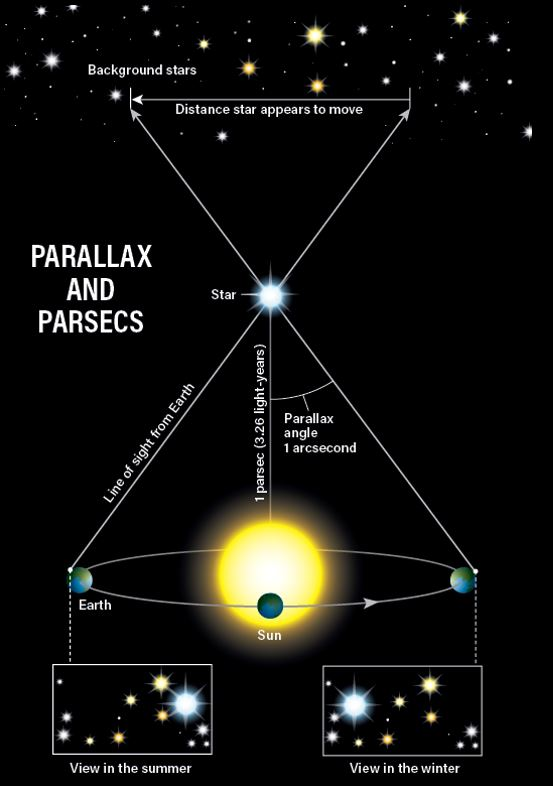
\includegraphics[width=8cm]{Parallasse.JPG}
\end{figure}

Per definizione un secondo d'arco
\textbf{ma loro hanno scritto "1 grado di quest'angolo" controlla}
porta a una distanza dal Sole di un parsec, che è equivalente 3.26 anni luce:

$$d\rm (pc)=\frac{1}{p['']} $$

Quindi la distanza in parsec è il reciproco dell'angolo di parallasse.

[Fa un esempio su Betelgeuse 1:41:00 circa fino a 1:46:30 ora mi siddiu]

Il metodo della parallasse ci permette di vedere corpi distanti fino a un massimo di 200 parsec, ma se vogliamo vedere più lontano si sono sviluppati vari metodi, che si rifanno però tutti alla relazione tra magnitudine apparente e osservata:

$$L_{\rm obs}=\frac{L_{\rm int}}{4\pi d^{2}}$$

Il metodo più utilizzato è quello delle cosiddette \textit{distanze spettroscopiche}: per una stella possiamo ottenere lo spettro (che ricordiamo essere la distribuzione dei fotoni con la lunghezza d'onda) e in esso possiamo identificare le righe spettrali; sulla base dell'intensità delle righe spettrali abbiamo attribuito alle stelle una temperatura; una volta conosciuta quest'ultima conosciamo la luminosità intrinseca dell'oggetto e possiamo confrontare questo valore con quello osservato, da cui ricaviamo la distanza a cui si trova la stella.

Questo metodo ci permette di arrivare a distanze di decine di migliaia di parsec, ma anche qui abbiamo dei limiti dovuti alla luminosità dell'oggetto: esso deve essere sufficientemente luminoso per poterne effettuare la spettroscopia, la quale prevede che il segnale venga "spalmato" in lunghezze d'onda, per cui dobbiamo avere un elevato numero di fotoni ad ogni lunghezze d'onda in modo da poter dare forma allo spettro. Ricordiamo infatti che il rumore è pari alla radice quadrato del numero di fotoni, per cui con un numero non sufficiente di fotoni la misura sarà indeterminata, il che vuol dire ad esempio che non vedremo le righe.

Allora è necessario a questo punto trovare qualcosa di meglio, che sia più efficiente della spettroscopia. Gli oggetti più adatti per questo compito sono le \textbf{stelle pulsanti}\footnote{Pulsare vuol dire che l'oscillazione è in risonanza con la lunghezza d'onda.}. Per valutare le distanze le più utili sono le Cefeidi. La caratteristica delle Cefeidi è che nel pulsare (quindi nel variare il loro raggio) presentano una differente luminosità e per determinarne la pulsazione possiamo misurare la magnitudine della stella. La differenza tra la spettroscopia è che in quest'ultima dobbiamo "spacchettare" tutti i fotoni per conoscere lo spettro, e quindi per ogni lunghezza d'onda dobbiamo avere un certo numero di fotoni e avremo eseguito una misura con una radice quadrata del numero di fotoni, mentre nella fotometria prendiamo tutti i fotoni e li mettiamo assieme, per cui possiamo avere una buona misura fotometrica di magnitudine anche con un oggetto debole cal punto di vista della luminosità.

Può accadere che, quando misuriamo una quantità nel tempo, questa presenti un carattere periodico, ed è proprio il caso delle Cefeidi: esse certo numero di giorni avranno nuovamente la stessa magnitudine (apparente). Si è poi scoperto che alcune di queste stelle presentano una luminosità intrinseca che dipende solo dal periodo, che permette di trovare la magnitudine assoluta (misuriamo la magnitudine apparente della stella, determiniamo il periodo e da questo determiniamo la magnitudine assoluta).

Nella figura seguente osserviamo la magnitudine di una stella in funzione del periodo:

\begin{figure}[H]
    \centering
    \includegraphics[width=8cm]{Magnitudine Cefeidi.JPG}
    \caption{Magnitudine Cefeidi}
\end{figure}

Generalmente, più è lungo il periodo, più è brillante la stella (il motivo è legato alla grandezza della stella: più è grande la stella, più sarà luminosa e maggiore sarà il periodo).

Esistono 2 classi di Cefeidi, quelle di tipo 1 e quelle di tipo 2. La definizione è legata alla popolazione a cui la stella appartiene: quelle di tipo 1 sono stelle di popolazione 1, con un'alta metallicità, mentre quelle di tipo 2 sono stelle di popolazione 2, con bassa metallicità. Con questo metodo otteniamo misure a distanze fino a 25 Mpc.

Esiste infine un altro metodo, quello delle \textit{supernove}, che però è casuale, possiamo misurare distanze solo quando avviene l'esplosione, quindi non è efficiente.

Nota: ogni metodo è testato sul precedente, cioè si fanno misure sugli stessi oggetti utilizzando i vari metodi.

\subsection{La Via Lattea}
Le stelle di cui abbiamo parlato non sono oggetti singoli, bensì sono spazialmente organizzati; la prova di questa affermazione è antica: guardando il cielo ci accorgiamo che non sono distribuiti uniformemente, sono raggruppati in una striscia, che è la via Lattea. Quando guardiamo la via Lattea in lunghezze d'onda diverse da quelle del visibile, vediamo che la galassia sembra cambiare forme:

\begin{figure}[H]
    \centering
    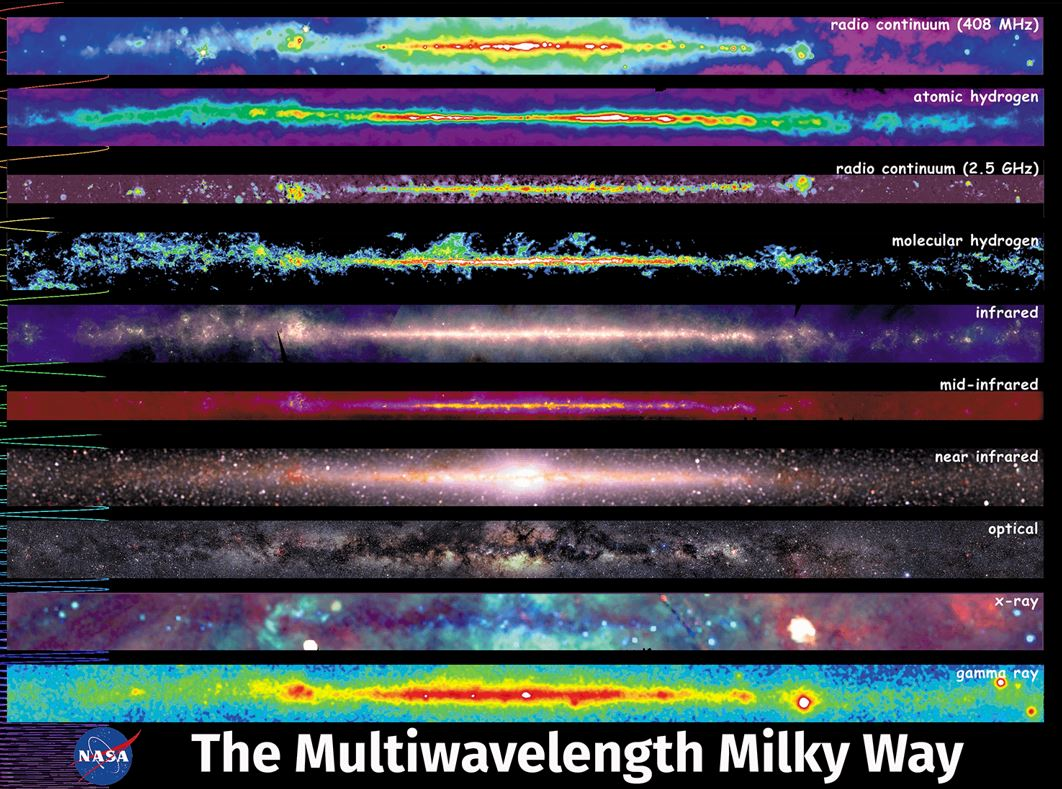
\includegraphics[width=10cm]{Via Lattea.JPG}
\end{figure}

Quindi, questa organizzazione delle stelle è qualcosa di più complesso che semplicemente "dove sono messe". Queste stelle sembrano occupare un volume che non è fatto solo di stelle, altrimenti le immagini sarebbero tutte uguali.

Il primo a scoprire che la via Lattea fosse fatta di tante piccole stelle fu Galileo, ma fu Immanuel Kant il primo a ipotizzare che la nostra galassia avesse una struttura planare (per cui la via Lattea è la visione di un oggetto planare, visto di taglio perché noi siamo all'interno). 
%e che qualche nebulosa potesse essere un'intera altra galassia.
Il primo che cercò di fare qualcosa dal punto di vista quantitativo fu Messier alla fine del '700: egli fece un catalogo in cui classificò i vari corpi; egli riportava gli oggetti ordinati per ascensione retta e a parità di questa per declinazione, dunque erano ordinati per posizione. Nei primi dell'800 Herschel incrementò il lavoro di Messier e catalogò 5000 oggetti. Herschel cercò anche di determinare la forma e la grandezza della galassia partendo da dalle assunzioni: tutte le stelle hanno la stessa luminosità e sono distribuite uniformemente nel cielo. Per ricavare la forma basta contare il numero di stelle in ogni direzione. In questo modo ottenne la seguente figura, dove il Sole era quasi al centro:

\begin{figure}[H]
    \centering
    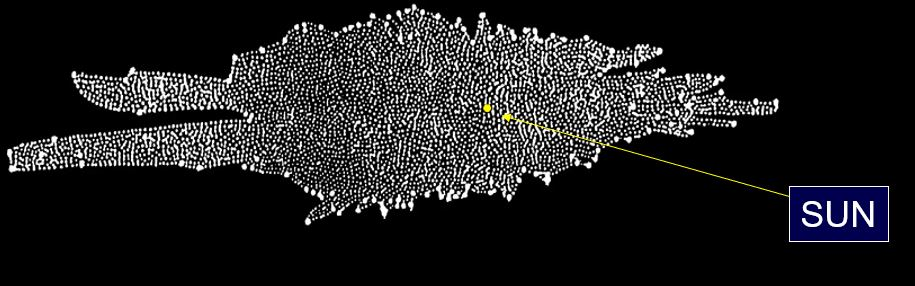
\includegraphics[width=10cm]{Via Lattea di Herschel.JPG}
\end{figure}

Questa fu la prima idea di Galassia, avente forma piatta e non a forma di disco, segno che ci sono delle zone in cui ci sono più oggetti. Il problema di questo modello è che Herschel non sapeva che lo spazio tra le stelle non era vuota e quindi non trasparente, per cui per lui non vedere una stella significava che non c'era, non che potesse essere oscurata da una nube ad esempio.

Una scoperta che ha rivoluzionato la visione della galassia è stata quella degli \textit{ammassi globulari}: oggetti sferici pieni di stelle. Questi oggetti devono stare per forza all'esterno della galassia perché sono troppo numerosi, e quindi si può immaginare che stanno orbitando attorno alla galassia, di conseguenza il centro della galassia sarà dato dal baricentro di tutti gli ammassi globulari. Il Sole così non si trovava più al centro della galassia, ma a 15 kpc da esso (ad oggi sappiamo che dista 8 kpc).

La scoperta fondamentale degli ammassi globulari è stata la composizione chimica di questi oggetti: essi hanno una metallicità inferiore a quella del Sole. Quello che è stato fondamentale per questi oggetti è stata la possibilità di confrontarli con il diagramma HR delle stelle che gli stanno attorno, questo ha permesso di scoprire che negli ammassi globulari non esistevano stelle di grandi massa, perché quest'ultime già si erano evolute dentro di essi. Di conseguenza essi permettono anche di dare una data agli oggetti. L'età degli ammassi è dell'ordine di 10 miliardi di anni.

Dopo aver visto forma ed età della galassia, possiamo misurarne la cinematica, cioè la velocità (sia radiale che trasversale, cioè il moto proprio) delle stelle, sfruttando l'effetto doppler. Come prima cosa possiamo per esempio misurare la velocità del Sole "a riposo", cioè rispetto alle stelle che lo circondano.

\begin{figure}[H]
    \centering
    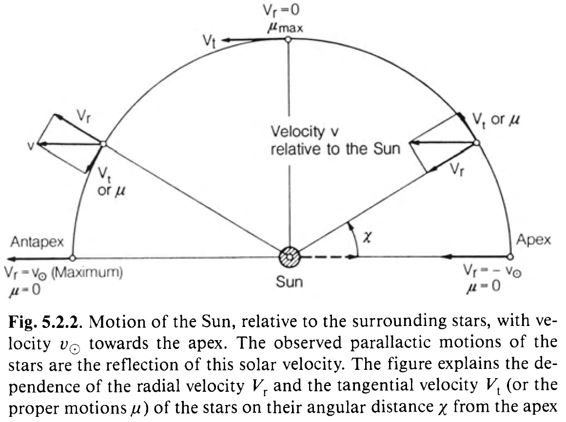
\includegraphics[width=10cm]{Velocita del Sole.JPG}
    \caption{Velocità del Sole}
\end{figure}

Rispetto alle stelle che lo circondano, il Sole in media si muove a 20 km/s nella direzione delle ore \textbf{CHE CAZZO VUOL DIRE}

\E stato poi introdotto un sistema di misura delle velocità che è nel sistema di coordinate galattiche, che vede un asse congiungere il centro della galassia e il Sole e sul piano perpendicolare all'asse, in senso antiorario, si misura la longitudine galattica, mentre l'altezza sul piano galattico viene chiamata declinazione galattica. La velocità possiede una componente radiale, rivolta verso il centro, che si chiama $U$, e una componente tangenziale (rispetto ad una eventuale orbita rispetto al centro della galassia) che si chiama $V$. Possiamo inoltre avere anche una componente perpendicolare che si chiama $W$, che serve a sapere se l'oggetto rimane sul piano.

Come si fa a capire come si muovono le stelle nella galassia? Quello che si è fatto è stato di determinare la cinematica di tutta la galassia cominciando a misurare le velocità di tutte e singole le stelle, usando l'ipotesi secondo cui tutte le stelle si muovono su orbite circolari e intorno al centro della galassia, su un piano detto piano galattico.

\begin{figure}[H]
    \centering
    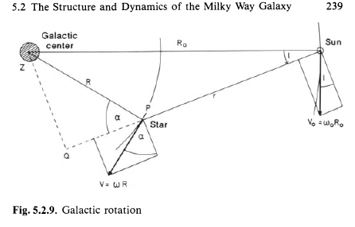
\includegraphics[width=10cm]{Dinamica della via lattea.JPG}
    %\caption{Dinamica della via Lattea}
\end{figure}

\rule[7pt]{\linewidth}{0.4pt}

\textbf{guarda Unsold pagina 382}

Parliamo della cinematica e della dinamica della via Lattea così come sviluppata da Lindblad e Oort nel 1926/27 nella loro teoria sulla rotazione differenziale del disco galattico. Supporremo innanzitutto che tutti i moti avvengano su orbite circolari planari attorno il centro galattico (indicato con Z).

\begin{figure}[H]
    \centering
    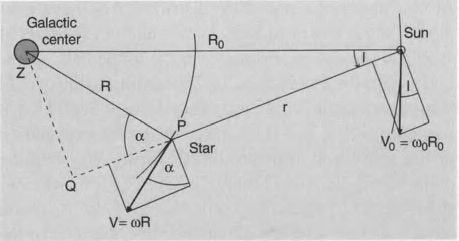
\includegraphics[width=7cm]{immagini/parametri_Oort_1.png}
\end{figure}

Sia $\omega=\omega(R)$ la velocità angolare di una stella P alla longitudine galattica $l$, funzione della distanza $R$ dal centro, allora $V=\omega R$ è la sua velocità lineare orbitale \textbf{ah??} sull'orbita galattica circolare. Invertendo tale relazione, per la velocità angolare e la sua derivata abbiamo

$$\omega=\frac{V(R)}{R}
\quad,\quad
\frac{d\omega}{dR}=\frac{1}{R} \left( \frac{dV}{dR} - \frac{V}{R} \right)$$

Per il Sole ($\odot$), poniamo $R=R_0$, $\omega(R_0)=\omega_0$ e $V_0=\omega_0R_0$. Detto precisamente, mettiamo sempre in relazione il moto a una media nelle vicinanze del Sole, che si chiama \textit{Sistema di Riposo Locale} \textbf{scrivilo meglio, secondo me non si capisce che è il nome della velocità media}, sottraendo il moto del sole da tutte le altre coordinate osservate.

Scomponiamo adesso la velocità relativa rispetto al Sole $\vec{V} - \vec{V}_0$ di una stella P nella componente lungo la congiungente $\rm \odot P$ e nella componente perpendicolare ad essa, in modo da ottenere la velocità radiale

$$V_r=V \sin{\alpha} - V_0 \sin l$$

e il moto proprio $\mu$ o la velocità tagenziale

$$V_t=V \cos{\alpha} - V_0 \cos l=\mu r$$

dove $r$ è la distanza della stella dal Sole. Possiamo eliminare l'angolo ausiliario $\alpha$ ponendo $\rm |ZQ|=R \sin{\alpha}$ e $\rm |PQ|=R\cos{\alpha}$, che possiamo ricavare\textbf{non sono sicuro di sta traduzione} dal triangolo $\rm \odot ZQ$:

$$R \sin{\alpha}=R_0 \sin l$$
$$R \cos{\alpha} + r= R_0 \cos{l}$$

Otteniamo

$$V_r=R_0(\omega - \omega_0) \sin{l}$$
$$V_t=R_0(\omega - \omega_0) \cos{l} - \omega r$$

Queste equazioni sono valide per stelle o gas interstellari in orbite circolari a distanze arbitrarie $r$ dal Sole.

Se consideriamo le vicinanze immediate (anche qua cerca un modo di dire più adatto) della Via Lattea, $r \ll R_0$, quindi possiamo usare l'espansione in serie

$$\omega - \omega_0
\simeq \left( \frac{d\omega}{dR} \right) (R - R_0)
\simeq - \left( \frac{d\omega}{dR} \right)_0 r \cos{l}$$

Introduciamo adesso le \textit{costanti di Oort} per la rotazione galattica differenziale:

$$A=-\frac{R_0}{2} \left( \frac{d\omega}{dR} \right)_0
=\frac{1}{2} \left[ \frac{V_0}{R_0} - \left( \frac{dV}{dR} \right)_0 \right]$$
$$B=-\frac{R_0}{2} \left( \frac{d\omega}{dR} \right)_0 - \omega_0
=\frac{1}{2} \left[ \frac{V_0}{R_0} + \left( \frac{dV}{dR} \right)_0 \right]$$

o anche

$$A+B=-\left( \frac{dV}{dR} \right)_0
\quad,\quad
A-B=\omega_0=\frac{V_0}{R_0}$$

dove abbiamo espresso le costanti usando le espressionidi $\omega$ e della sua derivata in termini di $V(R)$.

Con le costanti di Oort $A$ e $B$, l'approssimazione scritta poc'anzi e l'identità $2 \cos^2{l}= 1 + \cos{2l}$, la velocità radiale e quella tangenziale per i nostri dintorni, in funzione della longitudine galattica $l$, prendono una forma semplice:

$$V_r=Ar \sin{2l}$$
$$V_t=Ar \cos{2l} + Br$$

\begin{figure}[H]
    \centering
    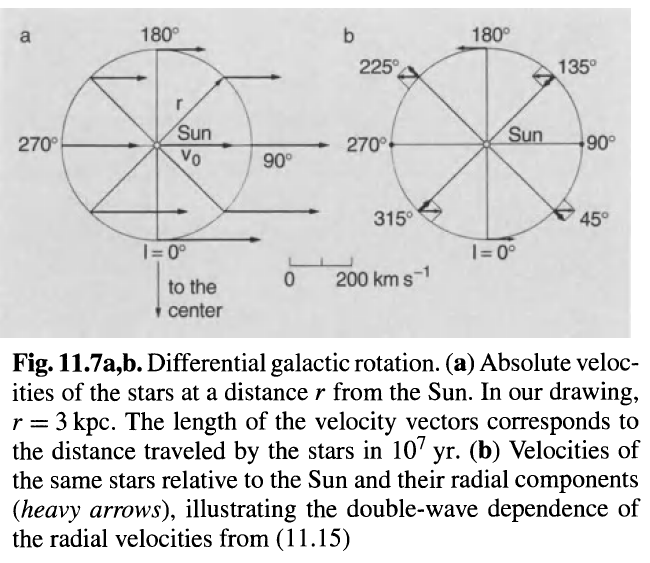
\includegraphics[width=7cm]{immagini/parametri_Oort_2.png}
\end{figure}

Dopo aver estrapolato la media dai moti peculiari, le osservazioni verificano questa "onda doppia" ($\sin{2l}$) delle due componenti della velocità molto bene. Mentre le ampiezze di $V_r$ e $V_t$ aumentano proporzionalmente alla distanza $r$, l'ampiezza del modo proprio $\mu=V_t/r$ è indipendente da $r$. I valori numerici delle costanti di Oort risultano essere:

$$A=\rm +14 \, km \, s^{-1} \, kpc^{-1}$$
$$B=\rm -13 \, km \, s^{-1} \, kpc^{-1}$$

Se avessimo considerato una rotazione rigida $(\omega=\omega_0)$, allora avremmo trovato $A=0$ $(V_r=0)$ e $B=-\omega_0$ $(V_t=-\omega_0 r \neq 0)$.

\rule[7pt]{\linewidth}{0.4pt}

Si nota che la galassia non è un rotatore rigido, cioè non tutte le stelle si muovono come se stessero su una ruota, questo è dovuto al fatto che la velocità angolare delle stelle è differente.

La velocità con cui il Sole ruota attorno alla galassia è di 220 km/s, il che implica che il periodo di rotazione dell'intera galassia è di 240 milioni di anni.

La domanda successiva a tutto ciò che abbiamo detto è: possiamo fare a questo punto una mappa della galassia? Il problema principale per fare ciò è dovuto al mezzo interstellare che assorbe la radiazione e ci impedisce di vedere lontano. Il meglio che possiamo fare è guardare alla lunghezza del radio poiché così l'estinzione risulta essere piccola. Tuttavia gli oggetti che emettono nel radio sono pochi (ricordiamo che l'emissione di corpo nero cade con la lunghezza d'onda, per cui non ci aspettiamo che un corpo come il Sole emetta nel radio), però esiste un processo fisico che ci ha permesso di fare la mappa della galassia ed è legato all'emissione di radiazione quando si ha quello che si chiama lo \textit{spin flip}\footnote{Se abbiamo un atomo di idrogeno in cui il protone ha gli spin allineati, ci troviamo in una configurazione a energia superiore rispetto al caso in cui l'elettrone ha spin opposto rispetto al protone} \textbf{nel dubbio cerca spin F su unsold pag. }, che permette l'emissione di un fotone di lunghezza d'onda 21 cm (vale per l'idrogeno neutro). Lo spin flip permette anche di fare una misura dei campi di velocità e inoltre ci ha fatto capire che le regioni di formazione stellare sono nei bracci di spirale. In queste regioni troviamo anche altri agglomerati di stelle, che sarebbero gli \textit{ammassi aperti}: regioni di formazione dove le stelle si sono appena formate e che possiedono tutte la stessa velocità attorno alla galassia (e sono costituiti da stelle "giovani").

Infine abbiamo il campo magnetico galattico. Per poter misurare questo campo magnetico si sfrutta l'effetto Faraday: se si ha radiazione polarizzata ed essa attraversa un mezzo dove è contenuto campo magnetico, la radiazione polarizzata gira il suo angolo. Ciò ci permette di studiare la variazione dell'angolo di rotazione e risalire al valore del campo (che è dell'ordine dei micro Gauss).

%If polarized radiation travels through a magnetic field, the direction of the polarization will rotate. The amount of such Faraday rotation is proportional to the component of the magnetic field parallel to the line of sight, number of electrons along the line of sight, distance travelled, and square of the wavelength of the radiation.

%More precise estimates of the strength of the magnetic field can be obtained from the rotation of the plane of polarization of the radio radiation from distant sources.

\textbf{RIASCOLTA E GUARDA LE ROBE COMMENTATE, sennò guardo Unsold 10.4.1 MA ANCHE MONACO PAG.92 CIRCA}

\subsection{La nostra galassia: finiamo il discorso della lezione precedente}
Abbiamo visto come un ammasso di stelle nel cielo è diventato una struttura, detta galassia. Essa è costituita da una serie di ammassi globulari, che sono grosse strutture costituite da centinaia di migliaia di stelle, che sembrano orbitare intorno ad un disco dove si trova la quasi totalità delle stelle. Tale disco è una struttura rotante su cui si trovano dei bracci di spirale. All'interno del disco sembra esserci un agglomerato sferico, detto \textbf{bulge}\footnote{Nota che, da questo momento in poi, quando parliamo di galassie, extragalassie, etc, spesso si utilizzano più termini per indicare la stessa cosa: il bulge (\textit{bulbo galattico}) sarebbe il nucleo.}, e si trovano le polveri da cui nascono le stelle.
%Questo è ciò che immaginiamo essere la nostra galassia come costituenti.
%Dimensioni $30 \, \rm kpc$.

In questo tipo di galassie convivono due popolazioni di stelle:

\begin{itemize}
    \item Popolazione 1, fatta da stelle calde, ricche di metalli, dislocate sul piano galattico;
    \item Popolazione 2 prive o quasi di metalli, vecchie, che sembrano orbitare attorno alla galassia.
\end{itemize}

Nel bulge convivono entrambe le popolazioni. Capire com'è distribuita la luminosità delle stelle nelle galassie, ci aiuta nello studio delle altre galassie. È necessario distinguere le porzioni, in quanto in esse ci sono caratteristiche cinematiche diverse: se guardiamo il disco avremo la velocità di rotazione dell'oggetto, se guardiamo il bulbo no. In una galassia a spirale come la nostra, la luminosità è concentrata sul disco. 

La nostra galassia è circondata anche da una struttura estesa e rarefatta (non più condensata in stelle), da un \textit{alone} (alone galattico), che sarebbe un mezzo diffuso, contenente anche stelle singole. Questa luminosità si vede chiaramente in galassie esterne alla nostra e prende il nome di "sombrero"; qui è evidente la luminosità diffusa che circonda l'intera galassia. L'alone della nostra galassia ha un diametro pari al disco ed è rotante come il disco. Le stelle interne all'alone hanno una cosiddetta cinematica "calda", cioè si muovono ad una velocità $di \sim 250 \rm \, km/s$, più alte rispetto a quelle delle stelle vicine che osserviamo in genere ($\sim 20 \rm \, km/s$) e esse orbitano ortogonalmente al disco. Nel disco distinguiamo, per la densità, due strutture cinematicamente diverse: disco sottile e spesso (il primo ha velocità più elevate).

Sorge un problema. Abbiamo realizzato una mappa della nostra galassia guardando le stelle. Osservando però il loro moto orbitale intorno alla galassia andiamo incontro ad un problema. Un oggetto orbita vedendo solo la massa che è presente dentro la sua orbita. Misurando la velocità delle stelle dal centro della galassia verso l'esterno, se la massa della galassia è costituita da stelle che stiamo vedendo ci si aspetta un certo andamento della velocità di rotazione delle stelle in base alla distanza dal centro (la velocità diminuisce allontanandosi). Dalla luminosità inoltre possiamo dedurre la velocità, questo perché c'è una relazione che lega luminosità e massa ($L \propto M^{3.5}$), e dalla massa possiamo dedurre la velocità orbitale che dovrebbe avere la stella. Questa cosa sembra però non funzionare: ci aspettiamo che gli oggetti più lontani ruotino più lentamente, ma ciò non accade per la nostra galassia.

Affrontiamo il problema. Il fatto che la velocità sia legata alla distribuzione della massa e che non diminuisca fa pensare che deve esserci, all'esterno della galassia, o all'interno che non vediamo, una certa massa che non è visibile con i nostri metodi standard (cioè a partire dalla luminosità). Questo andamento della velocità viene detto \textit{rotazione kepleriana}, e questa legge sembra abbiamo detto non essere rispettata, anzi si va verso un andamento costante della velocità.

Per risolvere, ci sono state due linee di pensiero:
\begin{enumerate}
    \item L'approccio seguito più dagli sperimentali, che iniziarono a parlare di materia oscura, cioè esiste attorno alla galassia della materia che non vediamo (appunto "oscura"), ma non torna bene con quello che è l'evoluzione stellare, ad esempio con i rate di formazione stellare (in una nube stellare si formano principalmente oggetti molto piccoli e poco molto caldi, quindi in giro non dovrebbero esserci molte stelle evolute). \E un approccio sperimentale perché si "ricerca" l'esistenza di tale materia;
    \item L'approccio seguito dagli studiosi più teorici, che aggiungono termini alla legge di gravità per far quadrare le cose.
\end{enumerate}

\subsection{Il nucleo della galassia}
Che cos'è il nucleo della galassia?

È un oggetto di densità incredibile, rimasto invisibile fino a pochi anni fa. Al suo interno (guardando a lunghezze d'onda di 90 cm) vediamo delle zone accese, tra cui la più brillante prende il nome di Sagittarius A, che dovrebbe essere il centro del tutto.

Il fatto che nel nucleo coesistano popolazione 1 e 2 è indicativo del fatto che c'è formazione di stelle. Ciò è strano, in quanto essendo una zona affollata è facile superare la massa di Jeans (che è la massa per cui una nube collassa, la quale ricordiamo essere direttamente proporzionale alla massa e indirettamente alla densità), ci aspetto un collasso della massa, ma anche la cinematica è elevata (o comunque lo è la temperatura, questo spiega perché non collassa).

È inoltre un luogo dove abbiamo tanta emissione radio. Quando l'emissione radio diventa significativa a livello di flusso non si può richiamare l'emissione radio del corpo nero\footnote{Se spostassimo il picco della planckiana nel radio dovremmo ridurre drasticamente la temperatura, e siccome il flusso va come $T^4$ non ci sarebbe emissione.}; si possono invece invocare meccanismi non termici di emissioni, che consistono in elettroni che ruotano attorno a campi magnetici ed emettono per sincrotrone. Il fatto che questo luogo sia così pieno di emissione radio fa pensare che ci siano elettroni liberi, i quali sono difficili da generare per cui serve un ambiente molto alto (penso intenda in temperatura) in modo da ionizzare tutti gli atomi per ottenerli, ed essi devono essere resi relativistici per far sì che emettano nel radio, quindi ci serve un meccanismo che ionizzi gli elettroni e li acceleri e in qualche modo producano sincrotroni. Tutto questo accade al centro della nostra galassia, ma perché? Cosa fa tutto questo?

Grazie all'attuale tecnologia, possiamo vedere nell'X la presenza di elettroni mediante l'emissione di sincrotroni nell'X. Il sincrotrone emette in tutte le lunghezze d'onda, ma poterlo vedere nell'X ha il vantaggio, rispetto al vederlo nel radio il quale non ha praticamente risoluzione spaziale, di vedere i dettagli di ciò che stava accadendo, in particolare si è trovata una temperatura dell'ordine di decine e centinaia di milioni di gradi. In definitiva, il centro della Galassia sembra essere un luogo dove accade qualcosa "di violento", con alta temperatura ed emissione radio. Questo si chiama \textit{Sagittarius A}.

Per determinare la massa di tutto questo si è fatto uso delle stelle che vediamo muoversi in orbita intorno al centro della galassia: per alcune stelle è stato possibile tracciare orbite e tramite queste determinare non solo il centro fisico della galassia, ma anche la sua massa. Il centro della galassia sembra essere fatto da milioni di masse solari, dovute al collasso di stelle che si sono unite. Questa massa non occupa uno spazio come lo intendiamo noi, ma dovrebbe essere un buco nero, cioè immaginiamo che Sagittarius A sia, di fatto, un buco nero. La nostra galassia sarebbe quindi costituita al centro da un buco nero. Qualche anno fa, grazie al Satellite Fermi, che ha come obbiettivo la misura emissioni gamma, ci ha informati del fatto che la nostra galassia abbia, ortogonalmente partendo dal centro, una struttura simile ad una clessidra caratterizzata dall'emissione di raggi gamma.

\subsection{Le galassie}

\epigraph{Uno pensa di essere unico, poi guardando scopri che non sei unico e che gli altri sono pure meglio.}{Ciccio pinguino}

\begin{figure}[H]
    \centering
    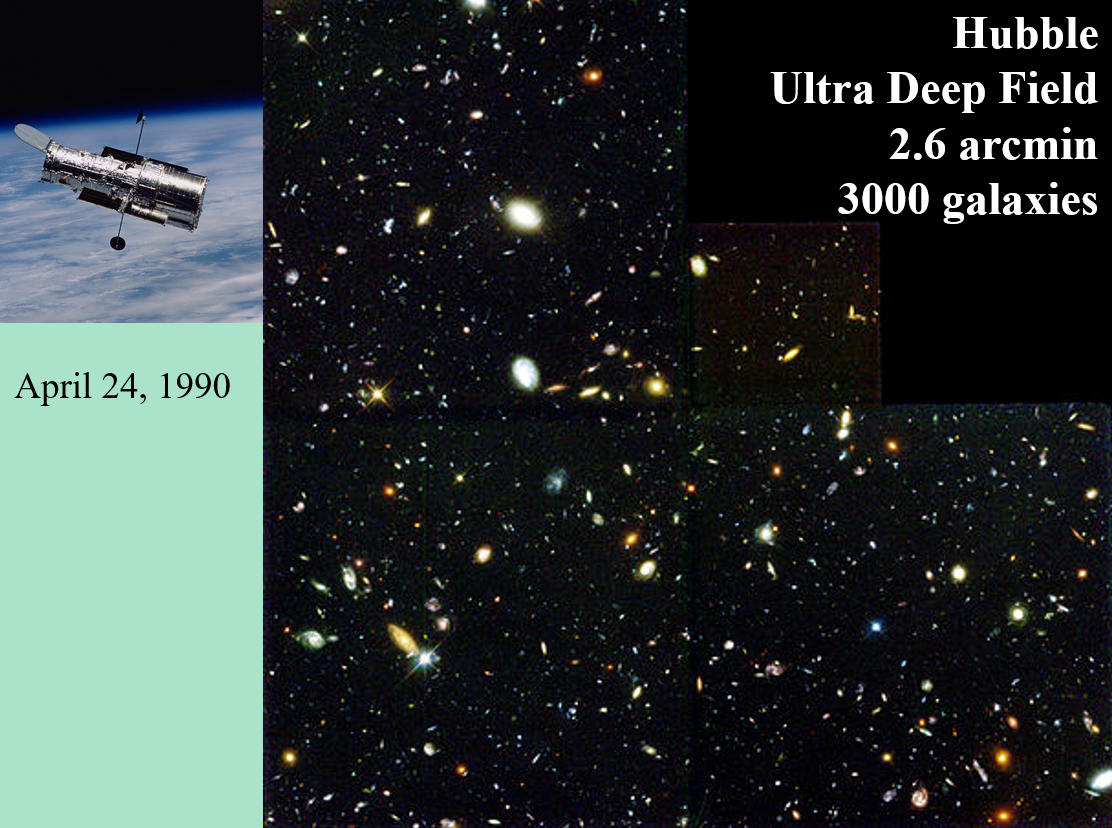
\includegraphics[width=0.5\textwidth]{immagini_lezioni12-12/hubble ultra deep field.png}
\end{figure}

La figura, che prende il nome di \textbf{Hubble Ultra Deep Field}, ci dice che in poco più di 2.6 arcmin\footnote{Per dare un'idea delle dimensioni ricordiamo che la Luna è 30 arcominuti.} ci stanno circa 3000 galassie, e sono tutte di forma diversa. Ciò pone una serie di problemi da risolvere.

Agli inizi del '900 non si aveva idea di quanto fosse grande la galassia, e nonostante si vedessero oggetti di forma diffusa genericamente chiamati nebulose, non si sapeva se queste stessero dentro o fuori la galassia, cioè se erano contenute o meno. Era difficile con gli strumenti dell'epoca (non si aveva abbastanza potere risolutivo).

Hubble fece fotografie di queste nebule, accorgendosi che in alcune di queste (o meglio nella direzione di queste) si trovavano oggetti che nel tempo variavano la loro luminosità. Scoprì che queste nebule possedevano delle stelle \textit{periodiche}, che variavano la loro luminosità periodicamente.

\begin{figure}[H]
    \centering
    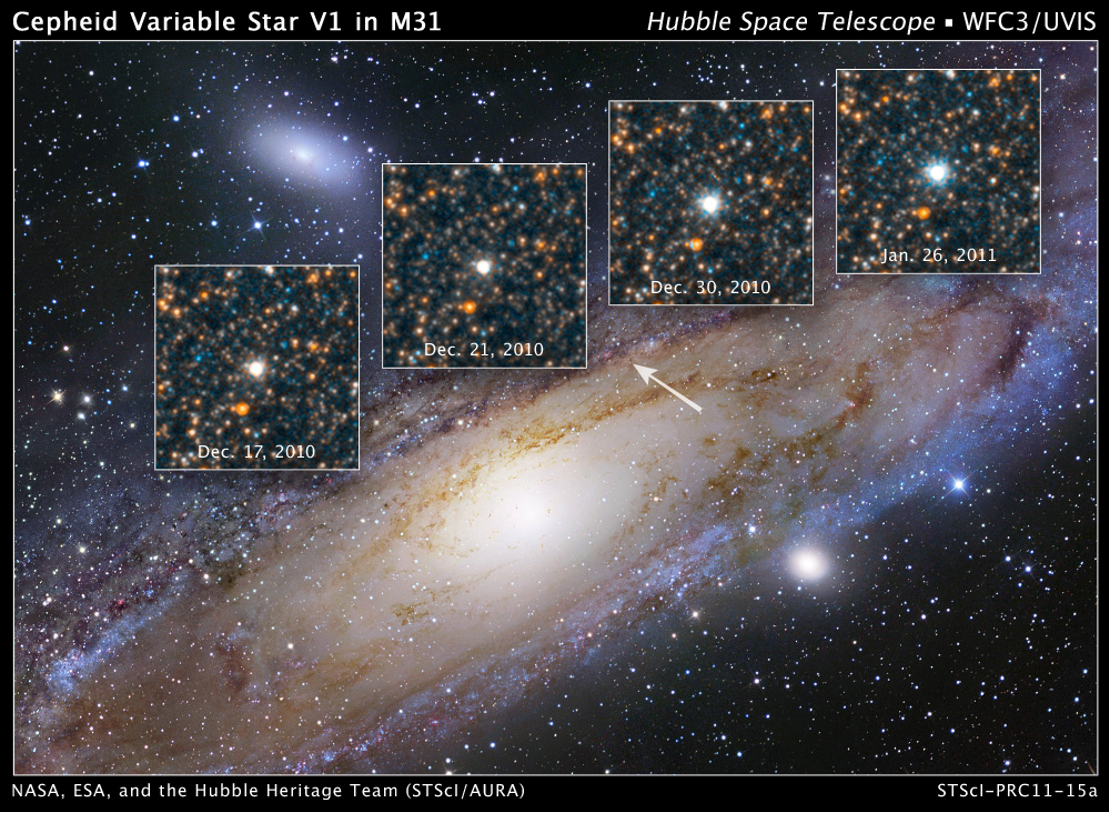
\includegraphics[width=0.5\textwidth]{immagini_lezioni12-12/stelle variabili.png}
\end{figure}

Si ricordò delle Cefeidi e attribuì alle Cefeidi una magnitudine assoluta, che poteva comparare con la sua misura, la magnitudine apparente. Da ciò, Hubble fu in grado di stabilire che questi oggetti erano molto più lontani della dimensione della nostra galassia, e quindi non appartenevano ad essa.

Il punto è che se conosciamo la dimensione di un oggetto e ne conosciamo la distanza, possiamo avere idea delle sue dimensioni lineari. Da ciò venne fuori che essi erano più grandi di quello che si pensava essere la nostra galassia.

Hubble, studiando le sue migliaia di foto, fece una classificazione, che vale ancora oggi, delle galassie, suddividendole in

\begin{itemize}
    \item Ellittiche;
    \item A spirale;
    \item Irregaolari
\end{itemize}

\begin{figure}[H]
    \centering
    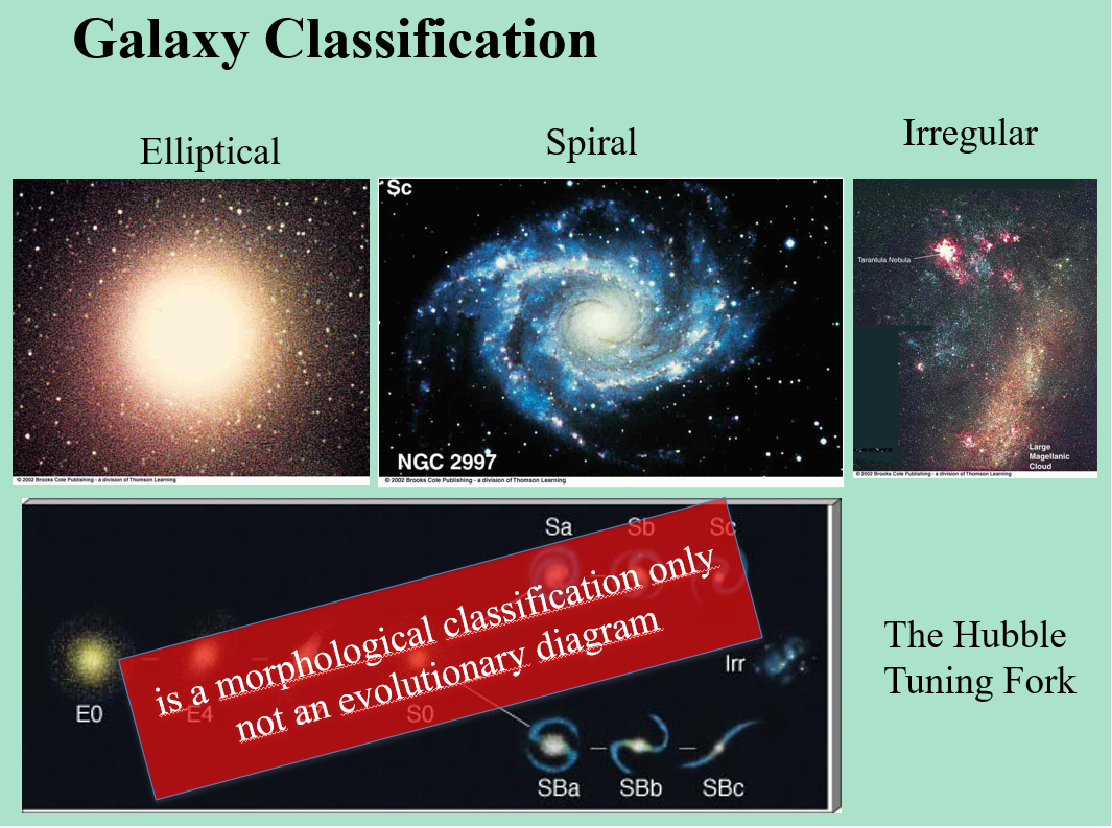
\includegraphics[width=0.95\textwidth]{immagini_lezioni12-12/classificazione galassie.png}
    \label{}
\end{figure}

Nota: Le galassie ellittiche sono degli ellissoidi/sferoidi, caratterizzate da una loro eccentricità.

\begin{figure}[H]
    \centering
    \includegraphics[width=0.5\textwidth]{immagini_lezioni12-12/eccentricità.png}
\end{figure}

Classificò questi sferoidi da un "$E0$" ad un "$E7$", dove il numero indica il valore dell'eccentricità moltiplicata per 10 (si poteva quindi andare da 0 (caso del disco) a 10 (caso di una sfera)). Questo schiacciamento di sferoidi può ovviamente essere l'effetto di proiezioni, quindi non è detto che quello che vediamo è davvero così.

\begin{figure}[H]
    \centering
    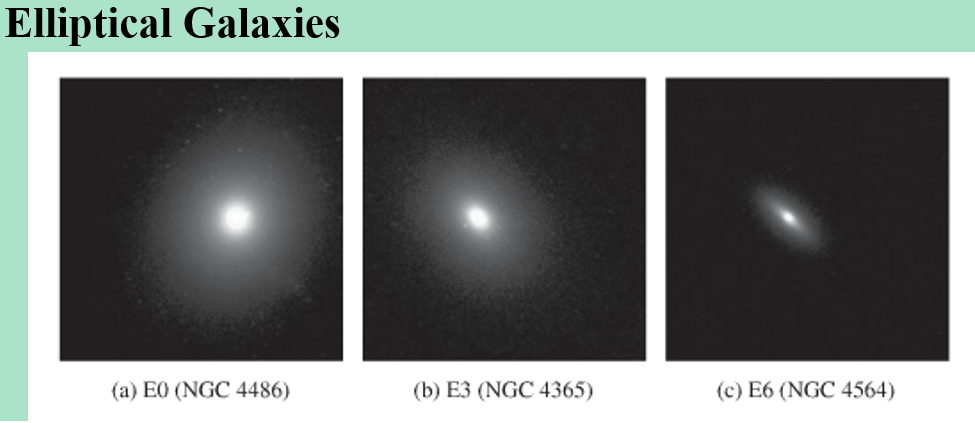
\includegraphics[width=0.7\textwidth]{immagini_lezioni12-12/galassie ellittiche.png}
\end{figure}

Inoltre divise le spirali in spirali e spirali barrate, le seconde aventi una barra che passa per il centro.

\begin{figure}[H]
    \centering
    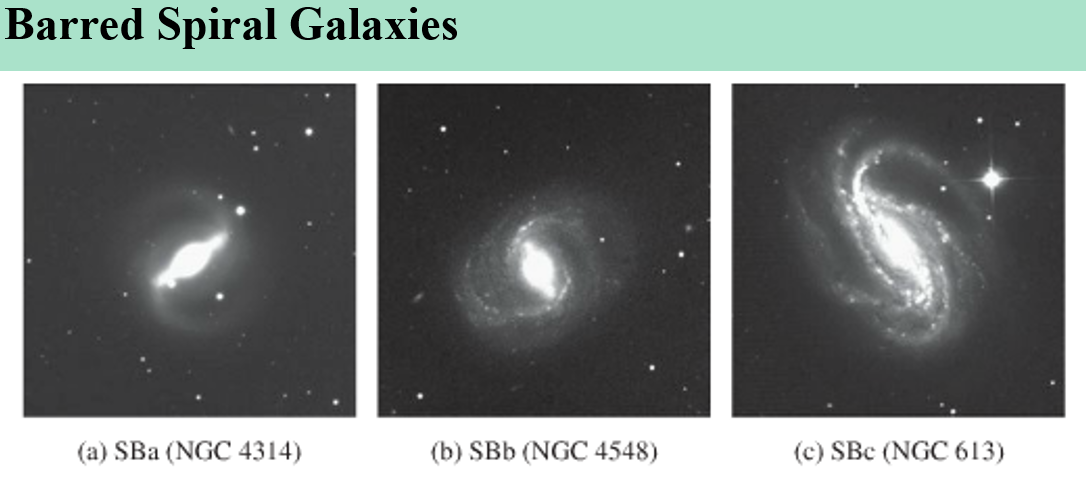
\includegraphics[width=0.7\textwidth]{immagini_lezioni12-12/galassie a spirali barrate.png}
\end{figure}

La nostra galassia ha una barra. Una spirale barrata si indica con $SB$; la nostra galassia è $SBb$ (continua a leggere e capisci).

Ancora, classificò le galassie a spirali in 3 gruppi ($Sa$, $Sb$, $Sc$):

\begin{itemize}
    \item quelle aventi spirali così strette da avvolgersi in se stesse;
    \item quelle intermedie;
    \item quelle le cui spirali non si chiudevano.
\end{itemize}

\begin{figure}[H]
    \centering
    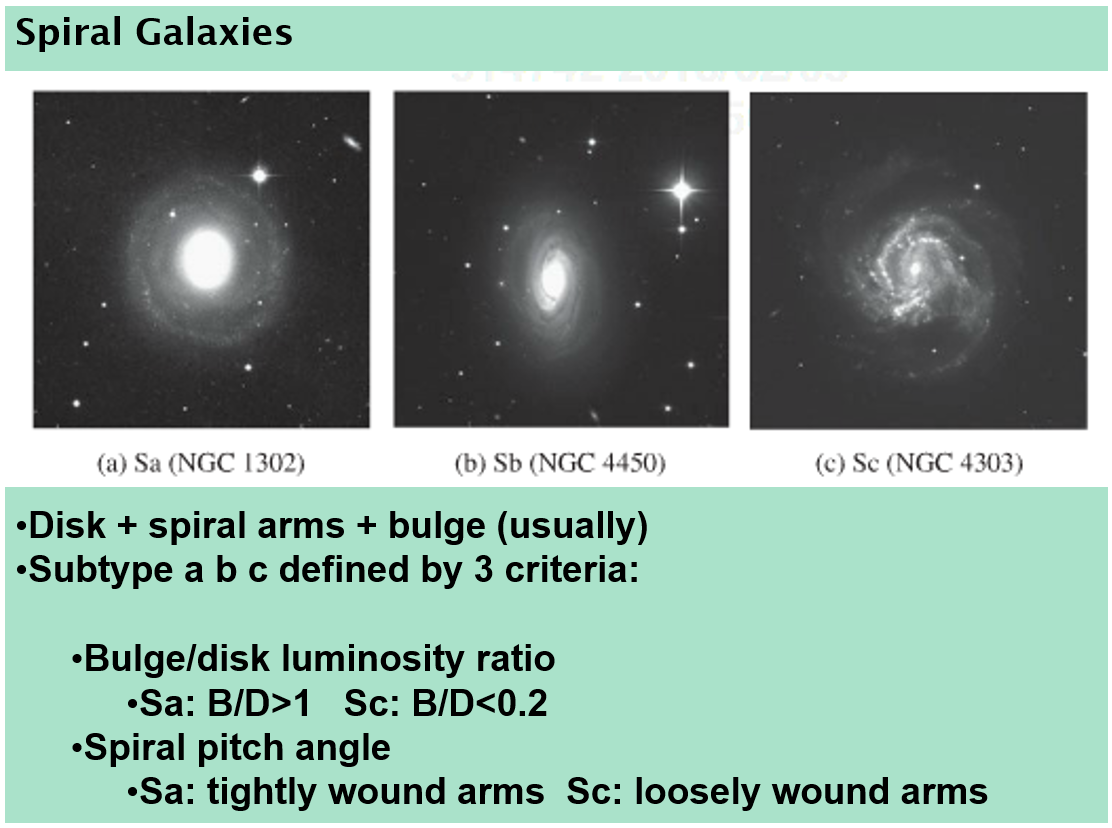
\includegraphics[width=0.7\textwidth]{immagini_lezioni12-12/galassie a spirale sa sb sc.png}
\end{figure}

Abbiamo detto che le galassie a spirali hanno un disco, le spirali ed un bulge. In base all'apertura o chiusura delle braccia (spirali), si può affermare che il bulge è più brillante del disco nelle galassie $Sa$ e minore in quelle $Sc$ (vedi figura sopra).

Le galassie a spirale sono, in numero, due terzi delle galassie totali. Sono ricche di polvere, gas, quindi si formano stelle; hanno dimensioni tra 10 e 30 kpc e massa tra $10^7$ e $10^{11}$ masse solari.

Sapere quanto è brillante una galassia permette inoltre di misurarne la distanza (si può immaginare che il rapporto tra brillanza del bulge e brillanza del disco sia un fenomeno fisico, che porta ad una luminosità predeterminata).

Abbiamo poi le galassie irregolari. Esse si immagina siano semplicemente il risultato della collisione di galassie. Tale idea nasce, oltre che da simulazioni numeriche, dal fatto che qui troviamo stelle giovani, cioè si stanno creando le condizioni per il collasso del mezzo interstellare, ad esempio per compressione.

Attenzione! Tutta questa è solo una classificazione morfologica e NON evolutiva.

Le galassie ellittiche sono centinaia di volte più grande di quelle a spirali.

Poi, Hubble fece una distinzione per queste che chiama "lenticolari" dal latino \textit{lens}, \textit{lenticchia}, un insieme di galassie più piccole, che sono dischi piccoli. Le galassie lenticolari, che chiama $S0$, sono piccole e non hanno struttura, non sappiamo cosa sono, e Hubble le mise nel mezzo perché pensava fosse una specie di fase per passare da spirali a ellittiche.

\begin{figure} [H]
    \centering
    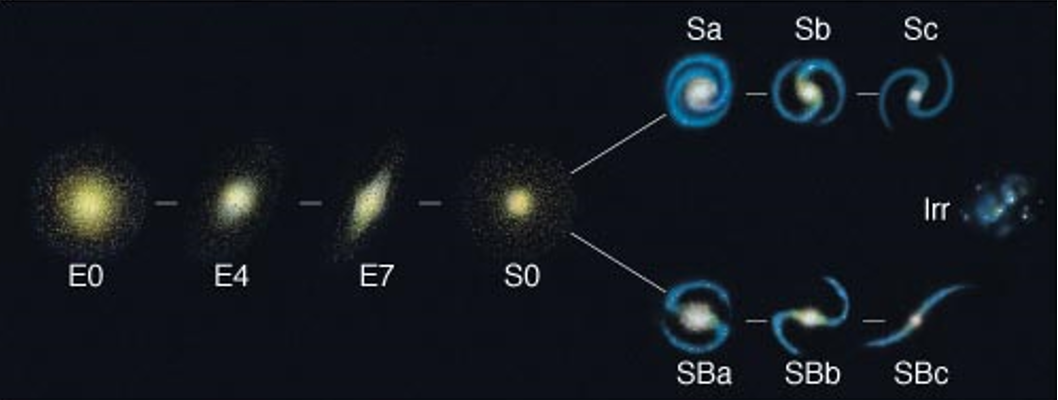
\includegraphics[width=\textwidth]{immagini_lezioni12-12/bho.png}
\end{figure}

Le Nubi di Magellano (\textit{Magellanic clouds}) sono due galassie che si muovono orbitando attorno alla nostra, così come le galassie M32 e M110 orbitano attorno ad M31. Esse sono il primo esempio di galassie esterne alla nostra. Da tali osservazioni concludiamo che le galassie sono organizzate in ammassi di galassie, cioè non stanno mai da sole. Tali ammassi sono fatti di oggetti che si muovono tra di loro, attorno al loro centro di massa (cioè gli ammassi sono autogravitanti).

\vspace{0.2cm}Ma come misuriamo le distanze tra galassie?

Si parte dall'andamento della curva della velocità delle stelle nelle galassie, la quale può essere ricavata per ogni galassia tramite uno spettrografo. Infatti, in uno spetto stellare, le righe spettrali si trovano ad una lunghezza d'onda che dipende dalla velocità, per l'effetto Doppler. Se facciamo uno spettro per ogni punto della galassia, troveremo delle righe, ma non alla lunghezza d'onda del laboratorio, bensì spostata; tale misura darà la componente della velocità della galassia che sta ruotando nella nostra direzione.

Misurando la velocità otteniamo una curva di questo tipo, dove al centro avremo la velocità di allontanamento dell'intera galassia, la parte che si allontana e quella che si avvicina.

\begin{figure}[H]
    \centering
    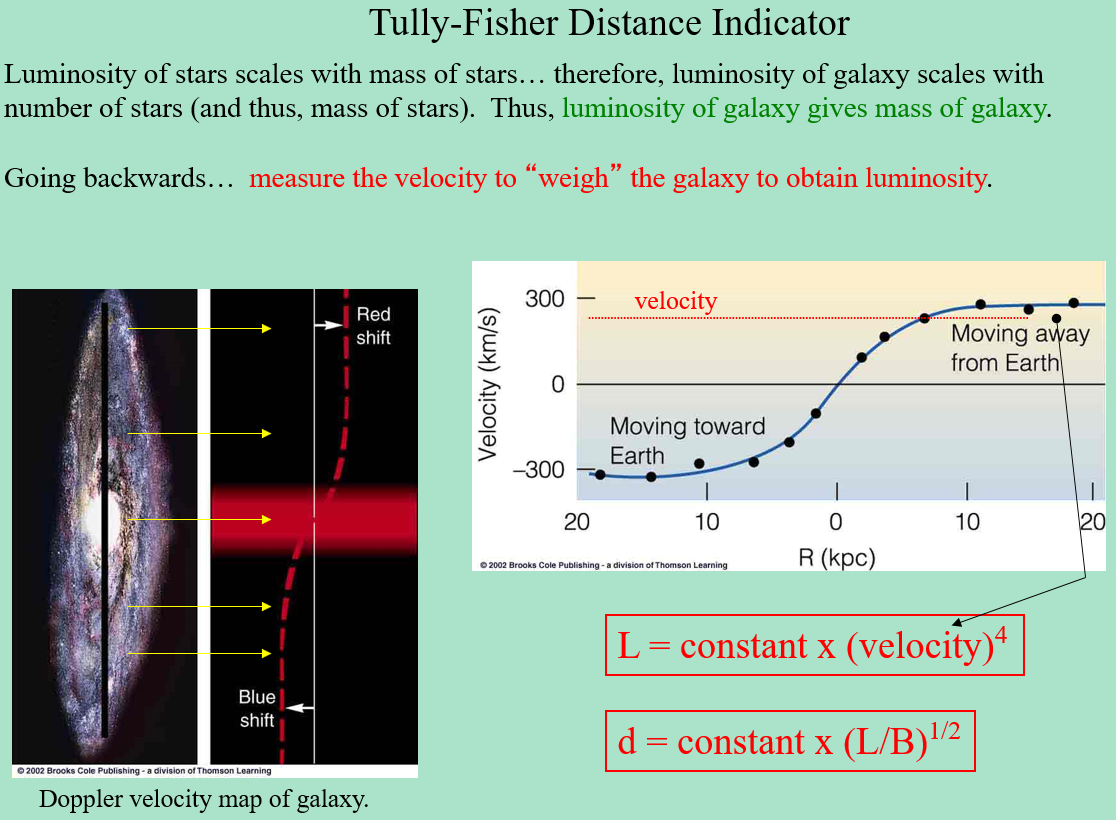
\includegraphics[width=\textwidth]{immagini_lezioni12-12/tully-fisher.png}
\end{figure}

Possiamo da qui stimare la massa della galassia. Per confronto con la nostra, possiamo stimare quale è la parte di massa della galassia responsabile di una emissione luminosa e attribuiamo alle galassie una luminosità intrinseca. La differenza tra luminosità intrinseca e quella che misuriamo dà un modulo di distanza. Questo metodo è stato immaginato da Tully-Fisher. È un metodo che ha tante ipotesi dietro e non è precisissimo, ma stima le distanze: con tale metodo si intende stimare l'ordine di grandezza della distanza.

Gli ammassi di galassie sembrano essere le strutture autogravitanti più grandi dell'universo. Un ammasso di galassie contiene da centro a mille galassie. Tra le galassie non vi è il vuoto, ma l' \textit{Intra Cluster Medium} (ICM), che è un plasma caldo con una grande quantità di materia oscura, invisibile. Vedremo che, per questo, tali ammassi sono sorgenti di Raggi X. Cercando di spiegare la dinamica degli ammassi, abbiamo bisogno, oltre che della massa luminosa, anche della dark matter, che ancora oggi si cerca, tuttavia non c'è ancora evidenza di quest'ultima.

Per avere un'evidenza della dark matter si parte dal presupposto di vedere radiazione elettromagnetica sotto forma di emissione gamma dovuta alla dark matter, ma nessuna misura effettuata su ammassi di galassie ha mai rilevato tale flusso di raggi gamma, finora è stata rivelata solo l'emissione X che è prova della presenza del plasma caldo; sono stati anche puntati telescopi X per rilevare le righe degli atomi che compongono il plasma, ma senza risultato.

Gli ammassi di galassie riportano quindi il problema della materia mancante, la grandezza di tali ammassi è di circa 1-5 Mpc.

Applicando il teorema del Viriale, supponendo di avere $N$ stelle con massa $m$, si potrebbe scrivere che l'energia cinetica $K$ dell'ammasso di galassie, che si muove in modo caotico \comment{(spiega la relazione usata per il valor medio di $v^2$)}, è proporzione alla massa $M=Nm$ per la dispersione delle velocità che misuriamo

$$K=M \langle v_r^2 \rangle=\frac{3}{2}M\sigma_r^2$$

dove $\sigma_r$ è la velocità media, supposta uguale in tutte e tre le direzioni. Applicando

$$2K+U=0 \implies 3M\sigma_r^2=\frac{3GM^2}{5R}\implies M_{vir}=\frac{5R\sigma_r^2}{G}$$

in questo modo possiamo ricavare la massa viriale misurando la velocità radiale di tutte le galassie di un ammasso, il che significa misurare il valore con cui la galassia si allontana, cioè la velocità media dello spostamento doppler.

Si può provare che la massa del viriale è confrontabile con la stima della massa che possiamo fare dalla luminosità ove possibile.

\vspace{0.2cm}Anche gli ammassi di galassie sono organizzati in ammassi; l'ammasso a cui noi apparteniamo è detto \textit{ammasso locale}. Quello che si percepisce è che il gruppo locale stia orbitando attorno al centro di un gruppo di ammassi detto \textit{SuperCluster}; noi apparteniamo a quello della Vergine, mentre a sua volta il supercluster fa parte di un gruppo ancora più grande; in generale noi apparteniamo ad una distribuzione di strutture non omogenea (sembra che ci sia una maggiore concentrazione su un piano detto \textit{piano supergalattico}), tra queste strutture sembrerebbe esserci del vuoto.

Tra gli oggetti più luminosi e più distanti ci sono le \textit{quasar}, ed essendo le più lontane sono anche le più veloci (Hubble misurò anche lo spostamento doppler delle galassie e scoprì che più un oggetto è lontano più è veloce); quando vediamo un oggetto che si allontana, il suo spettro si vede spostato verso il rosso, e questo quasar emette una riga spettrale dell'atomo di idrogeno tra livello 1 e 2 detta Lyman alpha, la quale però si trova a 4700 \A, e non a 1216 \A come di consueto, e ciò accade a causa della velocità del quasar; il mezzo che c'è tra la terra e il quasar è in grado di assorbire la radiazione emessa dal quasar, ma il mezzo si muove più lentamente del quasar, ogni pezzo del mezzo è responsabile di un assorbimento che dipende dalla sua velocità, dando origine alla \textit{Lyman Forest}. Possiamo quindi sapere come è distribuita la materia tra noi e il quasar per ogni lunghezza d'onda, cioè per ogni velocità e quindi per ogni distanza; con questo metodo di spettroscopia è stata dimostrata la presenza dei vuoti.

\begin{figure} [H]
    \centering
    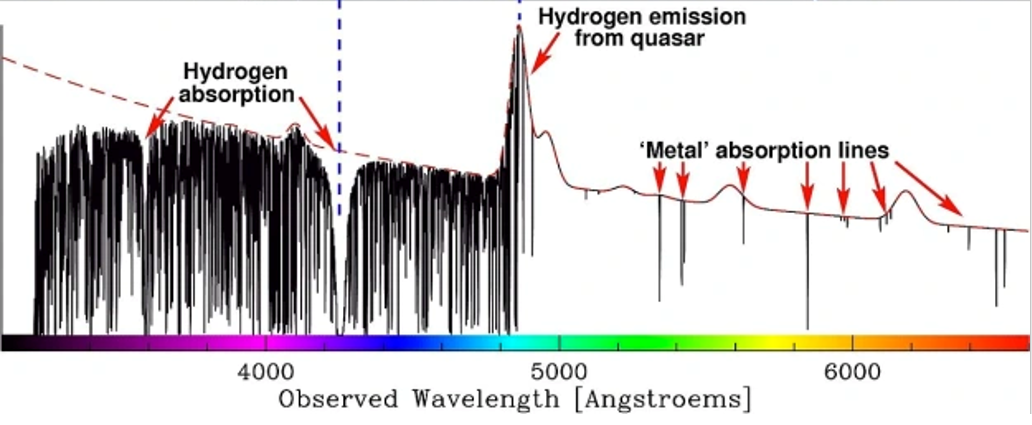
\includegraphics[width=0.9\textwidth]{immagini_lezioni12-12/44.png}
\end{figure}

\subsection{Nuclei Galattici Attivi e loro Classificazione}

Esistono galassie dove il nucleo è molto più brillante non solo del disco, ma ne esistono altre in cui è più brillante anche delle stelle che lo compongono, allora non è il contributo delle stelle che lo compongono a determinare la luminosità del bulge, si parla allora di \textbf{Nuclei Galattici Attivi}, detti AGN, regioni dalla luminosità non spiegabile dal contributo stellare; questi nuclei galattici attivi sono stati scoperti come delle sorgenti radio e poi divisi in \textit{Radio-Quiet} e \textit{Radio-Loud} a seconda della luminosità che si ha nelle regioni radio.

\begin{figure}[H]
    \centering
    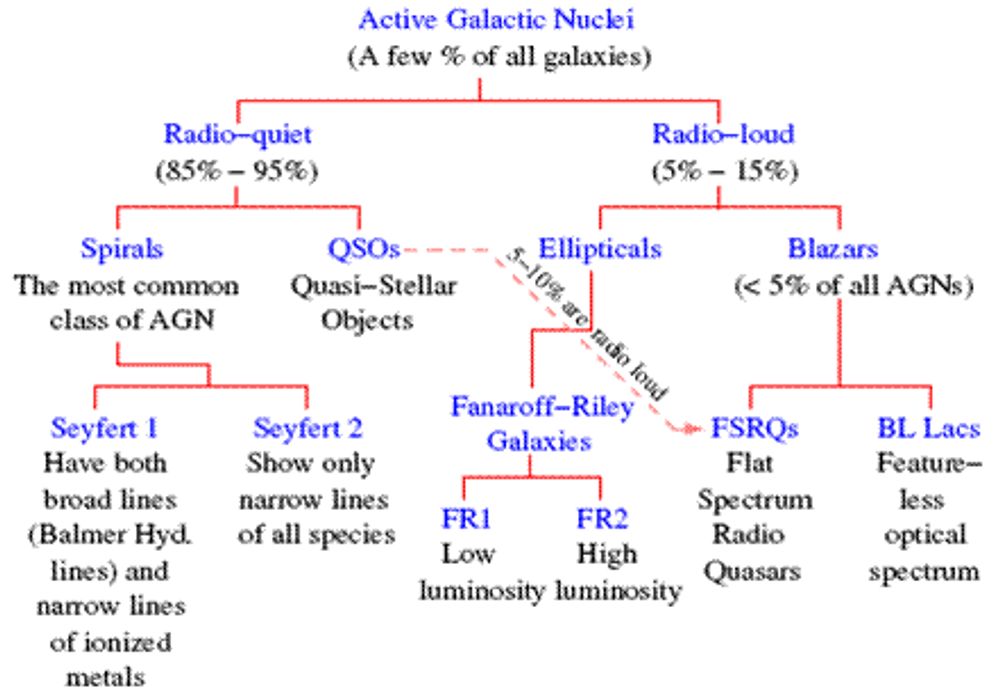
\includegraphics[width=\textwidth]{immagini_lezioni12-12/35.png}
\end{figure}

Le radio-quiet sono tipici delle galassie a spirale \textbf{o sono? aaaa}, come la nostra. Queste galassie vengono suddivise in \textit{Seyfert}1 e \textit{Seyfert}2: quelle di tipo 1 sono galassie con spettri con righe in emissione sia larghe che strette (in termini di lunghezza d'onda, credo intenda a lunghezze d'onda piccole e grandi), mentre quelle del secondo tipo presentano spettri con righe d'emissione strette; questi spettri non hanno nulla a che fare con l'emissione delle stelle, sono quelle del nucleo, infatti le righe che si vedono sono righe proibite (transizioni tra 2 livelli dove quello più alto è metastabile, cioè ha un tempo di decadimento molto lungo. Sono utili per determinare la densità di un gas); alcuni esempi di galassie Seyfert sono NCG-1566, NCG-7742 e la Circinus Galaxy, è interessante notare che la massa stimata per questi nuclei è di $10^6-10^7\,M_{\odot}$ e quindi probabilmente si tratta di un buco nero.

Un'altra categoria di galassie radio-quiet sono i \textbf{quasar}, termine derivante da "quasi-stellar-radio-sources", la cui luminosità intrinseca è di -32, contro -19 delle supernove. I quasar presentano una variabilità fotometrica; inoltre, come detto prima, le loro righe spettrali sono molto spossate verso il rosso (red-shift); questa proprietà è molto utile in cosmologia.

\textbf{definizione di transizioni proibite e semiproibite 2:03:00 circa}

Considerando ora le radio-loud esse si suddividono in \textit{Blazars} e galassie ellittiche; tra i blazar più famosi vi è BL Lac, che costituisce il prototipo di una categoria, ed è famosa perché non presentava nessuna riga rispetto al quasar; un'altra categoria di blazar è quella delle \textit{FSRQs} (Flat Spectrum Radio Quasars), dal nome si capisce che hanno uno spettro radio molto piatto. Per capire questa distinzione è necessario ricordare che negli oggetti ad alta temperatura (gli elettroni sono relativistici) i meccanismi di emissione sono di sincrotone o di Compton Inverso (un elettrone relativistico colpisce un fotone e lo sposta in lunghezza d'onda, facendo aumentare l'energia e con conseguente emissione di un gamma), nei blazars sono presenti entrambi, e la dominanza di uno processo rispetto all'altro stabilisce la classificazione, per cui la differenza fondamentale diventa l'intensità del campo magnetico dell'oggetto (se non c'è campo magnetico non abbiamo sincrotrone).

\begin{figure}[H]
    \centering
    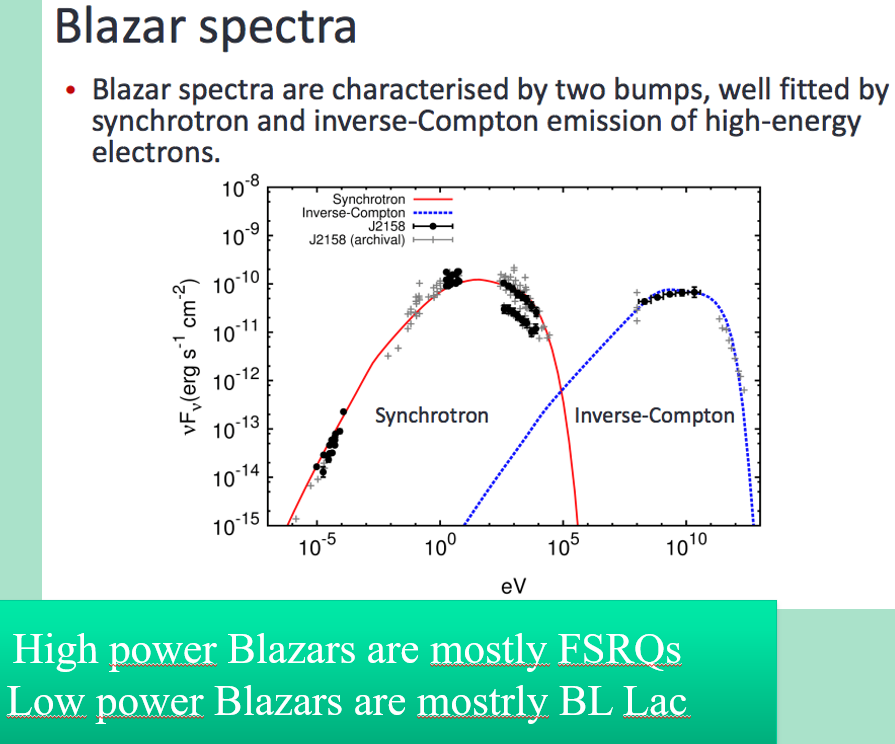
\includegraphics[width=\textwidth]{immagini_lezioni12-12/47.png}
\end{figure}

È importante sottolineare che in quasar e blazars non sappiamo cosa circonda il nucleo, forse la struttura esterna delle quasar è simile alle galassie a spirale e quella delle blazars alle galassie ellittiche.

Vediamo ora la categoria delle galassie ellittiche. Esse si suddividono in \textbf{Fanaroff-Riley 1} e \textbf{Fanaroff-Riley 2} a seconda della luminosità dell'oggetto e dalla forma dei jet (getti di radiazione elettromagnetica e particelle cariche): le prime hanno un jet molto sottile e brillante nella zona di emissione, mentre le seconde hanno un jet brillante sulla parte più esterna.

\begin{figure}[H]
    \centering
    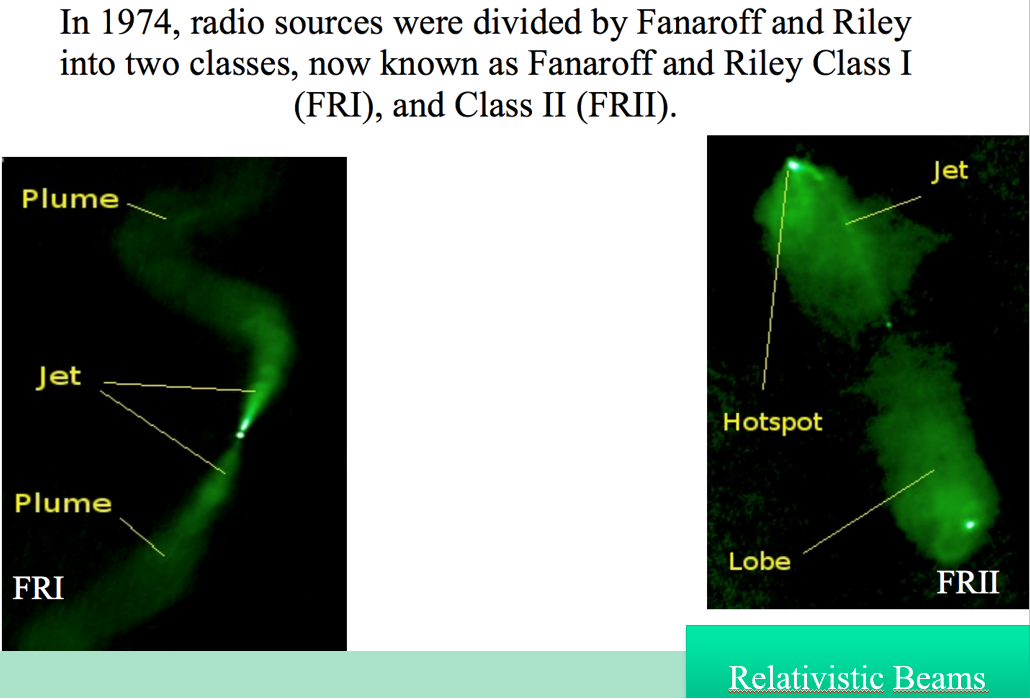
\includegraphics[width=\textwidth]{immagini_lezioni12-12/49.png}
\end{figure}

\subsection{Modello Unificato}
Ci sono oggetti celesti, come Centaurus A che non rientrano in nessuna delle categorie precedenti, tuttavia sembrerebbe che tutto quello detto finora si possa spiegare la teoria del Modello Unificato degli AGN, secondo la quale al centro della galassia si trova un buco nero (crediamo sia un buco nero per la massa stimata) che nasce dalla fusione di tante stelle, attorno a questo centro vi è un disco, dal buco nero diparte un jet.

\begin{figure}[H]
    \centering
    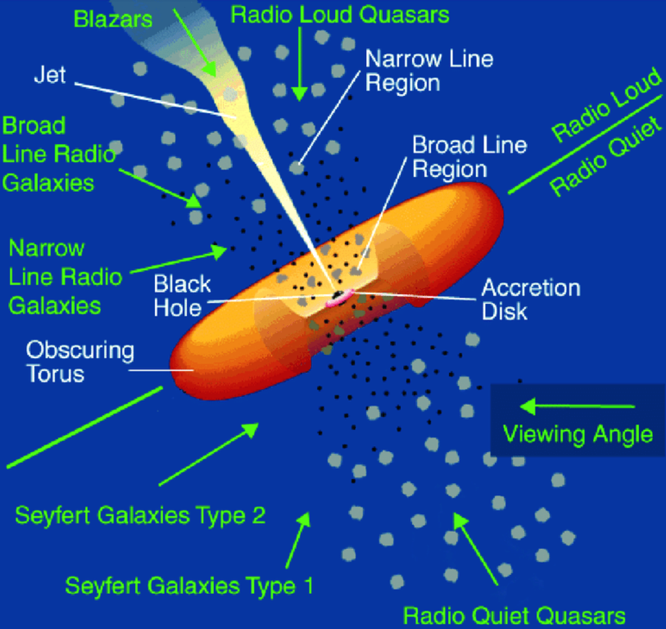
\includegraphics[width=12cm]{immagini_lezioni12-12/51.png}
\end{figure}

Con questa teoria, tutta la classificazione precedente è giustificata dalla direzione con cui viene guardata la galassia e dalle \textit{bubbles} intercettate (nella figura le bubbles sono quelle palline grigie o nere): guardando la galassia da una certa direzione potremmo vedere tanta emissione e quindi si ha una radio-loud, guardandola da un'altra potremmo vedere poca emissione, quindi sarebbe una radio-quiet ecc.

In definitiva, ogni categoria vista prima non è altro che una sfaccettatura dello stesso oggetto, che viene determinata dalla direzione di osservazione.

\subsection{Espansione dell'universo}

\subsubsection{Legge di Hubble}

Il problema di cosa fosse l'universo prende un aspetto scientifico soltanto nel '900, quando Hubble misurò la distanza delle galassie e come primo risultato mostrò che le nebule che si vedevano in cielo erano altre galassie. Egli misurò tali distanze a partire dalle misure di variazione di luminosità delle Cefeidi che erano legate ad una magnitudine assoluta. Inoltre egli ottenne gli spettri delle galassie, le quali hanno una emissione data dalla somma delle stelle che le costituiscono, per cui dal punto di vista spettroscopico si comportano come una sorta di "stella media". Egli trovò che le righe spettrali dell'idrogeno (le più intense) erano spostate in lunghezza d'onda rispetto a quella prevista.

Se supponiamo che questo spostamento sia dovuto all'effetto Doppler a causa delle velocità delle galassie, otteniamo velocità di migliaia di chilometri al secondo (molto maggiore di tutte le altre misurate nello spazio), che aumentavano con la distanza. Uno dei primi risultati della ricerca di Hubble è allora che l'universo si sta espandendo.

Ciò era stato previsto da Olbers nel 1800 per il fatto che il cielo di notte fosse buio. In un universo omogeneo infatti il numero di stelle aumenta col quadrato della distanza e sappiamo che la luminosità diminuisce anche col quadrato della distanza, quindi il cielo dovrebbe essere uniformemente luminoso. Olbers immaginò che il cielo fosse buio perché le stelle si allontanino con velocità diverse, e per spostamento doppler la loro luce visibile viene shiftata nell'infrarosso, quindi non la vediamo.

Nota: la differenza è che Olbers fece un ragionamento, Hubble portò una prova scientifica.

Hubble osservò inoltre che la velocità delle galassie aumenta linearmente con la distanza (secondo quella che sarà poi chiamata costante di Hubble $H_0$):

$$v=H_0 \cdot d$$

Il fatto che misuriamo velocità delle galassie che aumentano con la distanza potrebbe far pensare che la nostra galassia si trovi al centro di un sistema che si espande; in realtà la relazione di Hubble non ci rende un osservatore privilegiato perché se consideriamo il grafico seguente (supponiamo di essere fermi):

\begin{figure}[H]
    \centering
    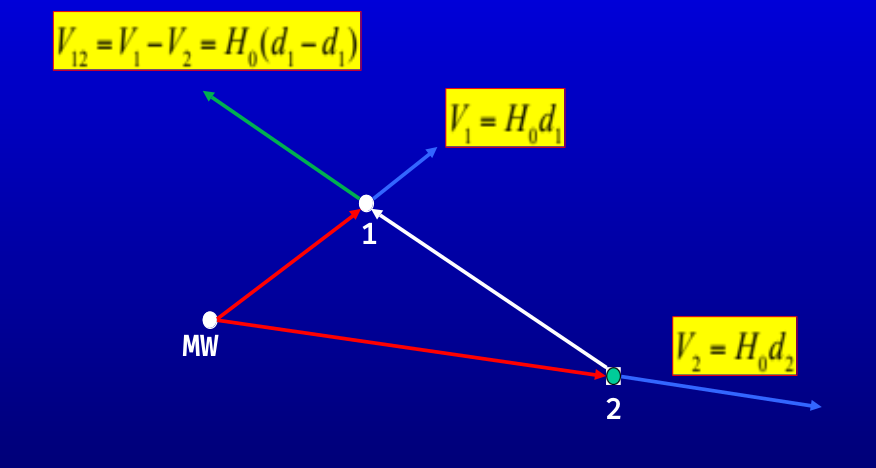
\includegraphics[width=0.5\textwidth]{immagini16dic/tuttilontani.png}
\end{figure}

\begin{itemize}
    \item Noi vediamo le galassie 1 e 2 allontanarsi;
    \item Un osservatore posto nella galassia 2 vede noi allontanarci (perché è in realtà lui che si allontana) e 1 allontanarsi;
    \item Un osservatore posto nella galassia 1 allo stesso modo vede noi e 2 allontanarci.
\end{itemize}

Paradossalmente allora tutti vedono allontanarsi tutti, dunque non esiste una delle 3 privilegiata. \E allora mantenuto il \textit{principio cosmologico}, che afferma che non esiste una posizione privilegiata nell'universo.

\subsubsection{Misura costante di Hubble}
Se supponiamo un espansione dell'universo a velocità costante, possiamo definire tempo di Hubble $T_0$:

$$T_0=\frac{d}{v}=\frac{d}{H_0 \cdot d}=\frac{1}{H_0}=14.4 \, \rm Gyr$$

che è una stima dell'età dell'Universo (cioè il tempo in cui "tutto era insieme"). \E in realtà un po' maggiore della migliore stima attuale (13,8 miliardi di anni) perché l'espansione non sembra essere stata lineare.

Il problema di misurare $H_0$ si riduce a misure di distanze e velocità. Hubble aveva i dati di 25 galassie che appartenevano tutte al gruppo locale, che essendo un ammasso di galassia è la struttura più grande che è gravitazionalmente legata, quindi le galassie hanno dei moti relativi tra loro: non sono ferme, si muovono risentendo del campo gravitazionale delle altre. Hubble quindi in realtà fece una misura di galassie che avevano un moto proprio, per cui il fatto che ad una certa distanza le galassie presentassero velocità diverse conteneva informazioni sulla dinamica delle galassie del gruppo locale. Non conoscendo tutto ciò, egli stimò inizialmente la costante valesse $H_0=500 \, \rm \frac{km}{s \cdot Mpc}$ e poi, osservando oggetti più distanti, trovò che $H_0=560 \, \rm \frac{km}{s \cdot Mpc}$. Oggi si misurano valori molto più piccoli (tra 50 e 100) e si utilizza in letteratura una media di $H_0=71 \, \rm \frac{km}{s \cdot Mpc}$. Con tale valore si stima un'età dell'universo di 13.8 miliardi di anni, valore che è consistente con le età che abbiamo determinato per gli ammassi globulare (con valore 500 l'universo sarebbe stato più giovane degli ammassi, il che creava un problema con i modelli)

Il problema dei moti relativi delle galassie locali si è parzialmente risolto misurando la velocità della nostra galassia rispetto a un punto più lontano e tenendone conto (più si guarda lontano e meno sono importanti gli effetti locali).

Se ci accordiamo sul valore della costante di Hubble, possiamo misurare distanze a partire dalla velocità di allontanamento delle galassie. Tale metodo ha portato ad un nuovo modo di definire lo spostamento doppler: noi siamo abituati a misurare la velocità come il rapporto tra la variazione della lunghezza d'onda e la lunghezza d'onda, moltiplicato per $c$, ma utilizzare l'effetto Doppler in termini della velocità di allontanamento è complicato perché si tratta di velocità grandi (c'è anche un fattore $c$). Si definisce piuttosto il parametro $z$ caratteristico di ogni oggetto spaziale attraverso cui si può ottenere facilmente la variazione di lunghezza d'onda.

\comment{\begin{figure}[H]
    \centering
    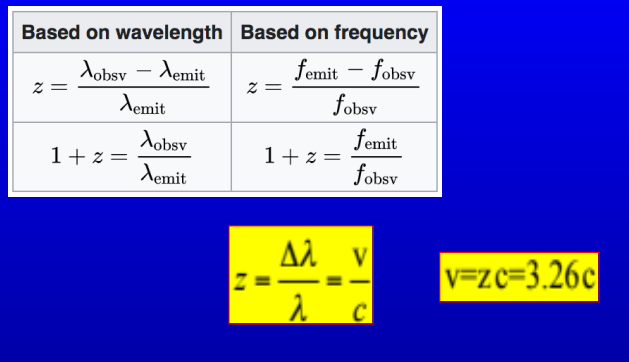
\includegraphics[width=0.8\textwidth]{immagini16dic/parametroz.png}
\end{figure}}

\begin{center}
    \begin{tabular}{|c|c|}
        \hline
        Basato sulla lunghezza d'onda & Basato sulla frequenza\\
        \hline
        &\\[-0.4cm]
        $\displaystyle z=\rm \frac{\lambda_{obsv} - \lambda_{emit}}{\lambda_{emit}}$ & $\displaystyle z=\frac{f_{\rm emit} - f_{\rm obsv}}{f_{\rm obsv}}$\\
        &\\[-0.4cm]
        \hline
        &\\[-0.4cm]
        $\displaystyle 1 + z=\rm \frac{\lambda_{obsv}}{\lambda_{emit}}$ & $\displaystyle 1+z=\frac{f_{\rm emit}}{f_{\rm obsv}}$\\[0.3cm]
        \hline
    \end{tabular}
\end{center}

$$z=\frac{\Delta \lambda}{\lambda}=\frac{v}{c}
\qquad
v=zc=3.26c$$

Il problema di misurare velocità in questo modo è che devono arrivare un certo numero di fotoni per misurare le lunghezze d'onda degli spettri con precisione.
Piuttosto si sono utilizzati dei filtri colorati per vedere a quale lunghezza d'onda cadesse la discontinuità di Balmer (Ricordiamo che essa è la lunghezza d'onda tale che i fotoni con lunghezza d'onda più corta (quindi con energia maggiore) sono in grado di ionizzare idrogeno. Normalmente è posta a 3667 \AA e per tutti i fotoni a $\lambda$ minori nello spettro di emissione si ha una totale mancanza), misurando il rapporto tra la luce osservate nelle bande e da lì stimiamo l'entità del redshift (photometric redshifts).

\begin{figure}[H]
    \centering
    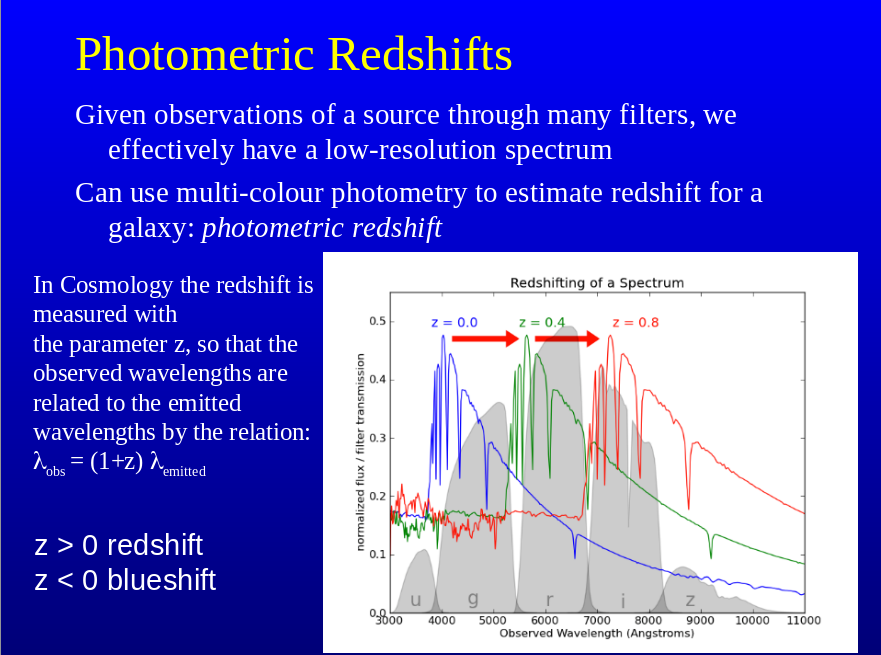
\includegraphics[width=0.5\textwidth]{immagini16dic/photoredshift.png}
\end{figure}

Con questi sistemi possiamo misurare oggetti lontani. L'oggetto più lontano si chiama z11 , ha redshift $z=11.09$ e età stimata $d=13 \; \rm Gly$ (miliardi di anni luce).

$z$ è legata all'età stimata (le galassie più lontane ci danno informazioni su un tempo più lontano) quindi possiamo studiare al variare di $z$ l'evoluzione dell'universo nel tempo.

\subsection{Storia dell'universo}
Da questo punto in poi parliamo di cosmologia, noi ci limiteremo ad alcuni accenni.

Innanzitutto, è importante sottolineare che l'espansione dell'universo non deve essere vista come una espansione di materia all'interno di uno spazio preesistente\footnote{Questo è il concetto opposto di universo, cioè l'universo definisce lo spazio.}, ma è esso stesso ad espandersi. Da questo punto di vista, la proprietà delle galassie di avere una velocità proporzionale alla distanza diventa una variazione della velocità dello spazio con la sua distanza da noi. Ciò viene normalmente visualizzato con un oggetto (nella figura ad esempio un cubo), dove la variazione delle distanze tra le galassie è conseguenza dell'espansione dello spazio che le contiene. Quindi in realtà le galassie non si stanno muovendo, ma sono trascinate dall'espansione dell'universo a cui appartengono, quindi si stanno muovendo indipendentemente da una forza, cioè non c'è nessuna forza che causa il moto, c'è semplicemente un fenomeno a cui gli oggetti sono costretti a partecipare perché contenuti.

Con questa visione, anche l'effetto Doppler cosmologico sarebbe dovuto all'allungamento (stretching) del campo di radiazione assieme all'universo. Ciò spiega perché esso è uguale in tutte le direzioni: perché l'espansione è isotropica (\textbf{magari rileggi})

\begin{minipage}{0.6\textwidth}
    \begin{figure}[H]
        \includegraphics[width=7cm]{immagini16dic/cubonero.png}
    \end{figure}
\end{minipage}
\begin{minipage}{0.4\textwidth}
    \begin{figure}[H]
        \includegraphics[width=5cm]{immagini16dic/waveshift.png}
    \end{figure}
\end{minipage}

Ripercorriamo la storia dell'universo:

\begin{itemize}
    \item Quale fosse la fisica quando tutto era concentrato in un punto non è noto
    \item solo dopo $10^{-32}$ secondi inizia a valere il principio di Heisenberg e la meccanica quantistica come la conosciamo. Si pensa che in questa fase ci sia stata una inflazione, cioè una rapidissima espansione durante la quale si sono iniziati a formare i primi agglomerati di particelle proprio per il principio di Heisenberg. 
    \item Calano la densità e la temperatura, si formano i protoni (a partire dai quark) ed entriamo nel mondo che possiamo testare in laboratorio.
    \item I protoni si raggruppano in elio 3 ed elio 4, poi anche in litio, berillio e boro, la quale abbondanza possiamo ora misurare e usare come verifica del modello (correggendo per la quantità di atomi che si sono formati successivamente). L'abbondanza del litio nella materia interstellare non è ancora ben spiegata.
    \item Siamo ancora ad una densità tale che gli atomi sono tutti ionizzati. Come accade nelle stelle, gli elettroni liberi aumentano l'opacità perché interagiscono continuamente con i fotoni
    \item Eventualmente (a 3000 kelvin) e si ha il fenomeno della \textit{ricombinazione}: protoni e elettroni si legano tra loro e si formano i primi atomi di idrogeno; a questo punto i fotoni interagiscono con l'idrogeno ionizzandolo e può capitare che quando il protone si ricombinerà con l'elettrone l'idrogeno che si forma non si trovi allo stato fondamentale, per cui decade per fluorescenza sul livello più basso emettendo nuovi fotoni a energie diverse che riescono a viaggiare e riusciamo a vedere tale flusso di fotoni. Il fatto che oggi vediamo la radiazione cosmica di fondo è un'ulteriore conferma di questo modello.
\end{itemize}

\begin{figure}[H]
    \centering
    \includegraphics[width=0.8\textwidth]{immagini16dic/bigbang.png}
\end{figure}

\subsection{Cosmic Background Radiation}
La visualizzazione di questi fotoni è avvenuta negli anni '60, quando due dipendenti della Bell furono incaricati di condurre uno studio sui disturbi delle emissioni radio. Essi scoprirono che ogni 24 ore arrivava un segnale radio (che corrispondeva a quando la Terra passava davanti al centro della galassia) e che tutto il cielo presentava una emissione radio; inoltre trovarono che in qualunque direzione dello spazio si guardi otteniamo una distribuzione che ricorda una plankiana tra intensità e lunghezza d'onda nelle microonde (escludendo le radiazioni degli oggetti cosmici classici). Essa è la radiazione di fondo delle microonde. La temperatura corrispondente a questa plankiana è di soli 2.725 K con delle variazioni di $\rm \mu K$ dovute alla interazione tra i fotoni e le galassie nel momento della loro formazione.

\begin{figure}[H]
    \centering
    \includegraphics[width=0.5\textwidth]{immagini16dic/cmbplank.png}
\end{figure}

Quello che sembra dunque è che l'emissione di fondo cosmico, che sono quei fotoni che cominciano ad andare in giro perché comincia a essere necessario del tempo affinché interagiscano con la materia, ci dà una prova del fenomeno del decoupling. \textbf{approfondisci}

Il fondo cosmico presenta una anisotropia locale di piccola scala: si hanno delle fluttuazioni del fondo che vengono imputate all'interazione tra i fotoni e le galassie, dunque all'interazione avvenuta quando si sono cominciate a formare le galassie\footnote{\E chiaro che i fotoni sono liberi di viaggiare se non incontrano una galassia}. Quindi la disomogeneità del fondo viene associata alla distribuzione delle galassie nell'universo.

\subsection{Cosmologia Newtoniana}

\textbf{GUARDARE MONACO}

Resta un'incognita: l'espansione dell'universo continuerà all'infinito?

Se immaginiamo l'universo come un pozzo gravitazionale possiamo immaginare che l'espansione continui se la velocità è maggiore della velocità di fuga.

%Dipende allora dalla densità dell'universo.
Usiamo la conservazione dell'energia classica (per questo cosmologia newtoniana):

$$\frac{1}{2}mv^2=G\frac{Mm}{r}$$

Ricordiamo $v=H_0 \cdot r$ per la legge di Hubble e supponendo che l'universo sia sferico e che l'universo è localmente indistinguibile da altri posti (quindi la massa è data dal prodotto della densità per il volume dell'oggetto) avremo:

$$\frac{H_0^2r^2}{2}=G\frac{\rho\frac{4\pi}{3}r^3}{r}$$

Possiamo definire la densità critica $\rho_c$

$$\rho_c=\frac{3H_0^2}{8\pi G}=10^{-26} \; \rm \frac{kg}{m^3}$$

Se $\rho<\rho_c$ l'espansione sarebbe infinita, altrimenti collasserebbe.

La stima attuale di densità è solo il 30\% di quella critica quindi l'espansione dovrebbe essere infinita. Se così fosse, l'universo si spegnerebbe (perché il motore di tutto è la gravità).

Misurare la massa comunque è molto difficile perché abbiamo informazione solo di quella che emette fotoni.

Posto $\Omega=\frac{\rho}{\rho_c}$ si hanno i vari modelli di espansione:

\begin{figure}[H]
    \centering
    \includegraphics[width=0.5\textwidth]{immagini16dic/cosmodelli.png}
\end{figure}

\begin{itemize}
    \item Se $\Omega<1$ l'universo non è legato, e si espande in eterno, seguendo una legge di tipo iperbolico;
    \item Se $\Omega=1$ l'universo è critico e l'espansione è ancora
    infinita;
    \item Se $\Omega>1$ l'universo è legato, e ricollassa su sé stesso ad un certo istante, in un Big Crunch.
\end{itemize}

Nel '98 Perlmutter-Ries-Schmidt scoprono che l'universo sta addirittura accelerando nella sua espansione il ché prevede l'azione di una forza di cui non sappiamo niente. In particolare trovano che la velocità misurata con la legge di Hubble è sistematicamente maggiore di quella misurata attraverso le esplosioni di supernove (non dice altro, probabilmente vuole dire che quella misurata con la supernova dipende dalla velocità nell'istante dell'esplosione mentre quella misurata da Hubble dipende dall'istante di misurazione).

Il fatto che l'universo acceleri porta inevitabilmente ad un aumento dell'energia. Come spieghiamo l'orbita delle stelle nella galassia con la materia oscura, in questo caso individuiamo la causa nell'energia oscura.

Si lavora con energie piuttosto che forze perché le forze sono vettori. L'energia di cui è costituito l'universo (contando la masse con $mc^2$) sarebbe solo il 5\% di quella necessaria a spiegare l'espansione dell'universo (nella diapositiva manca l'energia del campo elettromagnetico (fotoni) ma non sarebbe comunque sufficiente).

\begin{figure}[H]
    \centering
    \includegraphics[width=0.8\textwidth]{immagini16dic/tortauniverso.png}
\end{figure}